\makeatletter
\def\input@path{{./}}
\makeatother

\documentclass[12pt]{article}
\usepackage{palatino}
\usepackage[utf8]{inputenc}
\usepackage{enumitem}
\usepackage{setspace}
\usepackage{float}

\setlength{\topmargin}{-0.54in}
\setlength{\headheight}{12pt}
\setlength{\headsep}{20pt}
\setlength{\textheight}{9in}
\setlength{\textwidth}{6.5in}
\setlength{\oddsidemargin}{0pt}
\setlength{\evensidemargin}{0pt}


% Set PDF page size (for pdfLaTeX)
\pdfpagewidth=8.5in
\pdfpageheight=11in

\usepackage{amsmath, amsfonts, amssymb}
\usepackage{titling}

\usepackage{chicago}

\setlength{\droptitle}{-2cm}
\usepackage{graphicx}

\usepackage[breaklinks=true, colorlinks=false, urlcolor=black, linkcolor=black, urlcolor = black]{hyperref}
\usepackage{url}
\def\UrlBreaks{\do\/\do-}
\DeclareUnicodeCharacter{202F}{~}

\begin{document}

\begin{titlepage}
	\centering
	\vspace*{1in}

	{\LARGE Quantifying the Return on Investment of Campaign Contributions}\\[1.5cm]
	{\large Hope E.\ Mullins}\\[.5cm]
	{\large University of Central Florida}\\[.5cm]
	{\large Department of Economics}\\[.5cm]
	{\large 7/27/25}

	\vfill
	{\large ECO 6936}\\[.5cm]
	{\large	Capstone in Business Analytics}\\[.5cm]
	{\large Professor Harry Paarsch}\\[1cm]
\end{titlepage}


\doublespacing

\newpage
\section*{1 Introduction}

\indent Over the past fifty years, a succession of landmark Supreme Court decisions has reshaped the role of money in U.S.\ elections. In \textit{Buckley v.\ Valeo} (1976), the Court held that contribution limits --- though a restriction on political speech --- were justified by the government's interest in preventing corruption and preserving electoral integrity, yet it struck down aggregate expenditure limits because they violate the First Amendment's free-speech protections \cite{buckley1976}. More than three decades later, \textit{Citizens United v.\ FEC} (2010) overturned \textit{Austin v.\ Michigan State Chamber of Commerce} (1990) and parts of \textit{McConnell v.\ FEC} (2003), ruling that corporations and unions have a protected right to make independent expenditures in elections, a decision that ushered in the era of Super PACs and ``dark money'' (money given by nonprofits that are not mandated to disclose their donors) \cite{citizensunited2010}. In \textit{McCutcheon v.\ FEC} (2014), the Court further invalidated biennial aggregate limits on individual contributions (at the time, capped at \$123,200 per cycle\footnote{In 2014 USD.}), thereby granting wealthy donors greater flexibility in allocating funds across candidates and committees \cite{mccutcheon2014}. 

\indent These rulings, along with state-level reforms and evolving disclosure regimes, have produced a landscape in which electioneering mobilizes billions in fundraising each cycle. Yet, despite the scale of this spending, political actors, consultancies, and interest groups lack reliable ``return on investment'' (ROI) estimates that convert dollars into votes. From a campaign strategist's perspective, quantifying the marginal effect of an additional \$1 million on win probability or vote share is essential for allocating scarce resources effectively. Likewise, corporate and nonprofit donors need rigorous benchmarks to assess both whether and how to invest in candidates whose policy priorities align with their interests. Finally, voters themselves can benefit from transparent, data-driven insight regarding how spending sways electoral outcomes.

\indent Accordingly, I attempt to answer the following question: \begin{quote} \emph{How do the magnitude and composition of campaign contributions affect a U.S.\ House candidate's probability of winning and expected vote share?} \end{quote} In the following section, I review related empirical literature; in Section 3, I describe the theoretical frameworks, while in Section 4, I describe the database and data-processing steps. In Section 5, I present the econometric and machine-learning specifications, and in Section 6, I report results, interpreting the findings in Section 7 while discussing limitations in Section 8 and concluding in Section 9. In Appendix A, I document the filtering, cleaning, and inflation-adjustment procedures in detail, while in Appendix B I define variables, and in Appendix C I collect supplemental figures and tables.

\section*{2 Literature}

\indent For decades, many researchers have explored how campaign contributions affect electoral results, with a variety of focuses. In his 1978 study, ``The Effects of Campaign Spending in Congressional Elections,'' Gary Jacobson analyzed the relationship between campaign spending and electoral success, in particular highlighting the marginal effect of spending. Using regression analysis, Jacobson attempted to isolate the influence of campaign expenditures on vote share, finding a nonlinear, positive relationship between campaign spending and electoral success; the marginal effect of spending on vote share diminishes as the amount spent increases. Jacobson's findings challenged the idea that money alone can guarantee electoral victory under the argument that, while spending is influential, other factors such as candidate quality and party affiliation play significant roles in electoral outcomes \cite{jacobson1978}.

\indent To address endogeneity concerns that often arise when studying campaign spending, in his 1994 paper, ``Using Repeat Challengers to Estimate the Effect of Campaign Spending on Election Outcomes in the U.S.\ House," Steven Levitt focused on isolating causal effects. Typically, higher spending correlates with unobservable factors, making it difficult to determine the true effect of spending. Levitt compared ``repeat'' challengers --- candidates who run in consecutive elections (facing the same opponent) --- effectively controlling for variables like candidate quality and district characteristics that remain constant over time. The results show that money does indeed have an effect on electoral outcomes, but the impact is not large; the effectiveness of campaign spending depends significantly on context, such as the challenger's initial electoral position and the incumbent's strength, underscoring the limitations of financing \cite{levitt1994}.

\indent In ``Buying Supermajorities'' (1996), Groseclose and Snyder concentrated on the probability of achieving landslide margins, focusing not just on likelihood of winning but rather winning substantially. From their research, Groseclose and Snyder made many conclusions: campaign spending increases the likelihood of a landslide victory, but the relationship weakens after a certain level of spending; the impact of money varies depending on the strength of the incumbent and the competitiveness of the district; and the effectiveness of spending to secure supermajorities depends on the political context \cite{groseclose1996}.

\indent Building on his marginal-returns analyses, Jacobson (2004) revisited his research with two decades of additional data, introducing district fixed-effects, lagged vote-share controls, and spline specifications to confirm diminishing returns and differential effects for incumbents versus challengers \cite{jacobson2004}: money is a necessary but not sufficient condition --- candidate quality, district lean, and national tides remain dominant in determining vote share gains.

\indent Collectively, these studies share a number of core features, both substantive and meth\-o\-do\-log\-i\-cal. The researchers all employ regression techniques to estimate a ``dollars-to-votes'' relationship, taking explicit steps to control for confounders --- incumbency, district partisanship, candidate quality, and so forth. The research above, amongst others, documents clearly that challengers generally benefit more per dollar and that marginal payoffs shrink at high spending levels. These previous projects provide guidance for my own research.

\section*{3 Theoretical Framework}

\indent Several complementary perspectives frame how spending translates into electoral outcomes. First, microeconomic models interpret campaign spending as an input into a ``political production function'' or a ``political factory,'' where money buys votes \cite{jacobson1983}. Game-theoretic extensions cast these expenditures as bids in an ``all-pay auction,'' predicting sunk spending and strategic bidding \cite{Levin2004}. These approaches together forecast diminishing returns once campaigns saturate available media markets and core constituencies, and anticipate strategic spending patterns.

\indent Public choice theory refines the microeconomic view by emphasizing the incentives driving both donors and politicians. Contributions can be interpreted as investments --- donors channel resources into campaigns expecting future policy payoffs --- or as rent-seeking bids --- expenditures are sunk costs with no guaranteed return unless the supported candidate wins \cite{becker1983}. Under this lens, contributions reflect a rational actor's calculation of expected policy benefits net of bid expenditures; firms and interest groups will only invest in campaigns when anticipated returns exceed the cost of contributions. 

\indent Next, political science theories focus on how spending shapes voter behavior directly. Spatial utility models hold that voters choose the candidate closest to their own ideal point on an ideological spectrum \cite{downs2024}. Campaign resources, then, enhance a candidate's ability to convey issue positions accurately --- shifting perceived ideological distances and thus vote share. Similarly, persuasion theory argues that expenditures fund targeted messaging that can reframe issues, prime particular considerations, and activate latent preferences \cite{lupia2021}. Both perspectives suggest that money's effect is mediated through communication quality, media mix, and timing. 

\indent Finally, institutional theory adds another dimension by demonstrating how legal and regulatory structures alter the incentives and strategies surrounding campaign finance. Regulatory impact theory posits that contribution limits, disclosure requirements, and public-funding options change the ``production technology'' of campaigns by restricting inputs, increasing the cost of compliance, or shifting resources toward less-regulated vehicles \cite{stratmann2005}. For example, stringent contribution caps may drive donors toward independent expenditures or dark-money networks, reshaping the competitive landscape even if overall spending levels remain unchanged.

\indent Together, these theoretical lenses suggest a few key expectations for empirical analysis: diminishing returns, context-dependence, and strategic allocation. As established in the previous section, marginal vote gains per dollar spent, past a certain point in time, decline at higher spending levels. Moreover, the effectiveness of money varies by incumbency status, district competitiveness, and regulatory regime, also confirmed by earlier studies. Lastly, donors and campaigns allocate resources to maximize expected policy or electoral payoff, leading to heterogeneous spending patterns across races and over time. In the empirical work that follows, I draw on these frameworks to guide model specification and to interpret my estimates of the ROI of an additional million dollars in U.S.\ House political campaigns.

\section*{4 Data}

\indent My primary data source is DIME Public version 4.0 (Bonica), which ``contains over 850 million itemized political contributions made by individuals and organizations to local, state, and federal elections covering from 1979 to 2024'' \cite{bonica2024}. Given the magnitude of the data, I restricted my attention to U.S.\ House elections in cycles 2000 -- 2022 (2024 data was incomplete, as discovered during my cleaning process). Initial filtering uses DuckDB to select:

\begin{enumerate}
	\item Table \textbf{candDB}: federal House (\texttt{seat = `federal:house'}), \texttt{cycle} between 2000 and 2024, non-null \texttt{bonica\_rid}
	\item Table \textbf{contribDB}: matching \texttt{bonica\_rid}, \texttt{seat = `federal:house'}, \texttt{date} between 1998-01-01 and 2024-12-31\footnote{The date Jan 1, 1998 was used in attempt to capture pre-2000 contribution data for the 2000 election cycle.}\
	\item Table \textbf{donorDB}: matching \texttt{bonica\_cid} in contributions table
\end{enumerate}

\indent Variable pruning retains nineteen candidate-table fields: \texttt{bonica\_rid, bonica\_cid, \\ cycle, party, district, ico\_status, num\_givers, total\_unitemized, \\ total\_disbursements, total\_receipts, total\_indiv\_contribs, gwinner, \\ total\_pac\_contribs, total\_contribs\_from\_candidate, district\_pres\_vs, \\ total\_party\_contribs, ind\_exp\_support, ind\_exp\_oppose} \text{ and } \texttt{gen\_vote\_pct}. Nine contribution-table fields are kept: \texttt{cycle} (to validate the election year in the candidate table), \texttt{transaction\_type, date, amount, bonica\_rid, bonica\_cid, \\ contributor\_type, is\_corp,} \text{ and } \texttt{election\_type}. All other columns within these tables are dropped, and the donor table is removed entirely.\footnote{No variables related to my objective were contained within this table.} A description of all variables, as well as how they were transformed for modeling, if applicable, is located in Appendix B.

\indent Joining candidate and contribution tables yields approximately 97.4 million rows. I kept only general-election observations (\texttt{election\_type = `G'}), drop rows with null \texttt{gen\_vote\_pct} or \texttt{gwinner}, and then drop remaining nulls in \texttt{transaction\_type, date, contributor\_type}, and \texttt{district\_pres\_vs}, leaving 9,430,440 observations. I then converted \texttt{is\_corp: `corp' $\xrightarrow{}$} 1, NULL $\xrightarrow{}$ 0.

\indent Finally, I attached a CPI deflator table (base 2024 USD), adjusted all monetary columns accordingly, computed each contribution's \texttt{days\_before} (days between contribution date and election date), dropped original money and date fields, and encoded categorical variables: \texttt{contributor\_type} $\xrightarrow{}$ binary, one-hot for \texttt{ico\_status}, and frequency encoding for \texttt{transaction\_type}. The resulting {\tt house} table is ready for aggregation and modeling.

\subsection*{Visual Analysis}

Figure~\ref{fig:dist} depicts the distribution of logarithmic-scaled contributions in the cleaned table. It illustrates the heavy right tail --- most contributions are small, but a few very large gifts stretch the distribution. This indicates that contributions made by individuals may play a greater role in affecting election outcomes compared to committees, loans, and candidate self-financing.

\begin{figure}[h]
	\centering
	\includegraphics[width = 0.7\linewidth]{../Figures/amount_dist.pdf}
	\caption{Log-scale Contribution Relative Frequency Distribution}
	\label{fig:dist}
\end{figure}

Figure~\ref{fig:trend} depicts total U.S.\ House campaign contributions (in 2024 USD billions) by cycle. An upward trend is apparent, demonstrating the rise in campaign financing over recent years and thus the value in quantifying how a candidate's likelihood of victory changes as donations increase.

\begin{figure}[!t]
	\centering
	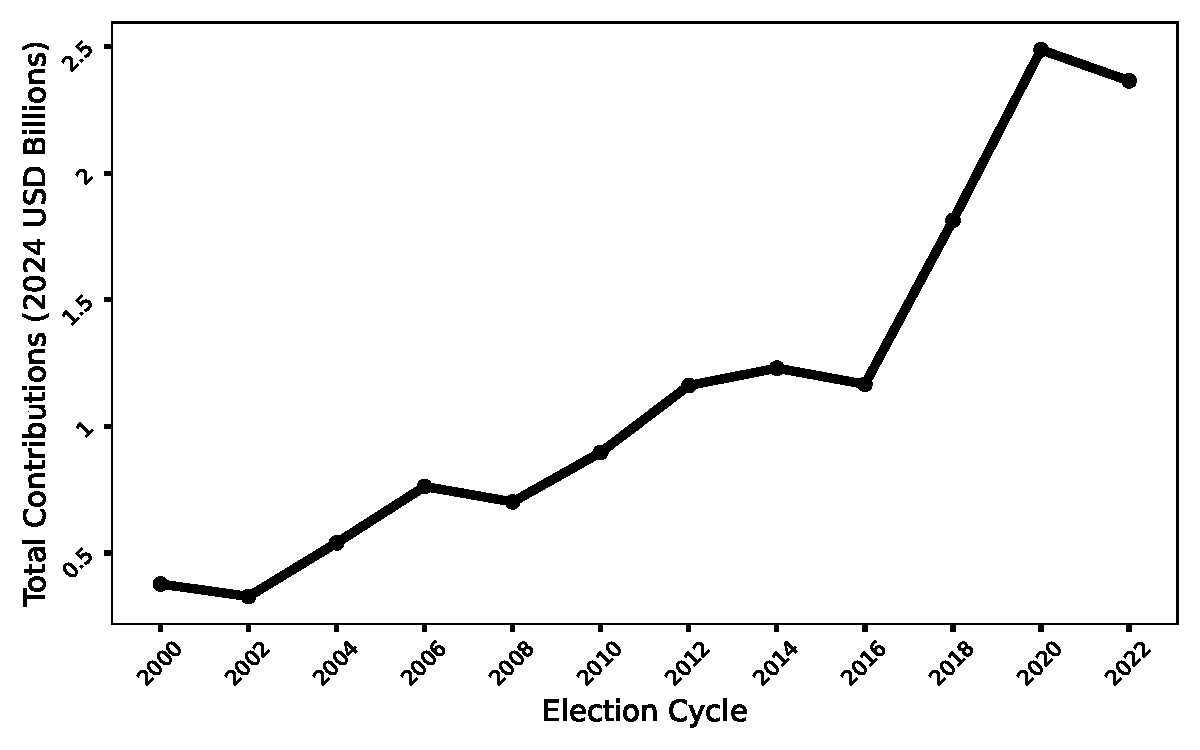
\includegraphics[width = 0.7\linewidth]{../Figures/cycle_spending_trend.pdf}
	\caption{Total U.S.\ House Campaign Contributions by Cycle (2024 USD Billions)}
	\label{fig:trend}
\end{figure}

\section*{5 Empirical Specifications}

\subsection*{5.1 Data Aggregation and Feature Construction}

\indent Using DuckDB (script \texttt{aggregation.py}), for each cutoff $X$ in $\{360, 240, 120, 60, 30, 14, 7, \allowbreak 1\}$ days before election, I aggregated all contributions with $\texttt{days\_before} \ge X$ into one candidate-cycle record.\footnote{Given my presumption that the marginal ROI across time would not be constant, building models based on where in the campaign a candidate is (timing-wise) is important. Essentially, this script is an automated process allowing the user to choose any cutoff date and generate a model at that cutoff.} For each $X$-day window I selected, I computed: \( \texttt{n\_contribs}_{X}\); \(\texttt{avg\_tx\_freq}_{X}\) (from frequency-encoded \texttt{transaction\_type}); \texttt{district\_pres\_vs}; \\ \(\texttt{indiv\_mill}_{X}\), \(\texttt{comm\_mill}_{X}\), and \(\texttt{corp\_mill}_{X}\) (million-dollar sums of individual, non corporate-committee, and corporate-committee contributions, respectively); \texttt{num\_givers}; \texttt{total\_receipts}; \texttt{ind\_exp\_support}; \texttt{ind\_exp\_oppose}; \texttt{party} dummies; \texttt{ico\_status} dummies; \texttt{incumbent}; and outcome (\texttt{gwinner} or \texttt{gen\_vote\_pct}).

In summary, this script builds snapshot aggregates for particular cutoff periods before the election. For straight logistic and linear regression, the individual, non-corporate committee, and corporate-committee monetary components add up to the total amount a candidate received by that point in time. Therefore, when calculating the ROI from each of these components, total ROI may be calculated by adding the independent effects. Alternatively, in the generalized additive models to follow, total ROI is a weighted combination of the individual marginal effects.

All aggregated tables are written to Parquet for reproducibility.\footnote{Parquet is a columnar storage file format optimized for efficient data processing, particularly in big data environments. I utilized this because I was unsure how large my aggregated data files would end up being.}

\subsection*{5.2 Logistic Regression for Win Probability}

For each cutoff, I fit a logistic regression of the form

\[ \Pr (W_n = 1) = \operatorname{logit}^{-1} \Bigl[ \beta_0 + \sum_{k \in \{\mathrm{indiv}, \mathrm{comm}, \mathrm{corp}\}} \beta_k \log(1 + \mathtt{k\_mill}_X) + \boldsymbol{\beta}_4^\top \mathbf{Z}_n \Bigr], \]

\noindent where $\mathbf{Z}_n$ includes standardized controls: number of contributions, average transaction type frequency, number of givers, independent support spending, independent opposition spending, district-level Democratic presidential vote share, party, and incumbency status.

\indent I trained on a 75 percent stratified random split, standardized via \texttt{StandardScaler}, and fit \texttt{sklearn.LogisticRegression} (L2, $C = 10^6$).\footnote{The parameter C is set to approximate unregularized MLE; many errors arose during pure logistic regression. This choice renders regularization negligible in practice.} Out-of-sample performance is assessed by ROC--AUC, accuracy, and recall. Total return on investment was computed by summing the three spending coefficients (those for individuals, non-corporate committees, and corporate committees) for a \$1 million log-bump at the sample mean and then exponentiating for the odds-ratio (script \texttt{model\_logistic.py}).

\subsection*{5.3 Logistic GAM for Win Probability}

To capture potential nonlinearity, I fit a logistic generalized additive model,

\[ \Pr (W_n = 1 ) = \operatorname{logit}^{-1} \Bigl[\beta_0 + \sum_{j} s_j (X_{nj}) + \sum_{\ell} \gamma_\ell F_{n \ell} \Bigr], \] 

\noindent where $s_j (\cdot)$ are penalized splines on each log-transformed spending and continuous control, and $F_{n \ell}$ are the categorical indicators. Smoothness is selected by grid-search on the training fold; evaluation uses the same 75:25 split and metrics as in the MLE logistic regression. Derivatives calculated at the mean recover a ``GAM-ROI'' log-odds slope for \$1 million (script \texttt{model\_logisticGAM.py}). 

\subsection*{5.4 Ordinary Least Squares Regression for Vote Share}

For each cutoff, vote share $\mathrm{VS}_n$ is modeled as

\[ \mathrm{VS}_n = \alpha_0 + \sum_{k} \alpha_k \log(1 + \texttt{\textit{k}\_mill}_X) + \boldsymbol{\alpha}_4^\top \mathbf{Z}_n + \varepsilon_n, \]

\noindent with the same $\mathbf{Z}_n$ controls as used in both logistic regressions. I fit a least-squares model using \texttt{sklearn.LinearRegression}, as well as report out-of-sample $R^2$, RMSE, MAE, and 5-fold cross-validated $R^2$. To try to improve predictive performance, I also ran Ridge and LASSO regularization over a logarithmic grid of penalty factors (25 alphas from $10^{-3}$ to $10^3$, selecting by CV). For interpretability, I tabulated standardized coefficient magnitudes (absolute values) to rank feature importance and plot their trajectories across cutoffs (on a log scale). Additionally, I produced a heatmap of least-squares $p$-values (for key predictors) to illustrate how statistical significance varies with time.

\subsection*{5.5 Linear GAM for Vote Share}

I fit a linear GAM,

\[ \mathrm{VS}_n = \delta_0 + \sum_{j=1}^p s_j(X_{nj}) + \sum_{\ell=p+1}^K \delta_\ell\, X_{n\ell} + \varepsilon_n, \]

\noindent with penalized splines on each continuous predictor and linear terms for categorical variables (script \texttt{model\_linearGAM.py}). Smoothing penalties ($\lambda \in [10^{-2}, 10^3]$) were selected by repeated $k$-fold CV; out-of-sample $R^2$, RMSE, and MAE are reported. ROI was computed by finite differences on each spending spline at the mean and weighting by the average spending mix, yielding $\Delta \mathrm{VS}$ per \$1 million.

\medskip
\indent All coding was completed in Python 3.11, using DuckDB for aggregation, \texttt{pandas} and \texttt{numpy} for processing, \texttt{scikit‑learn} for the logistic, OLS, and regularized fits, and \texttt{pygam} for all GAMs. Visualizations are generated with Matplotlib (and Seaborn for the least-squares $p$‑value heatmap).

\section*{6 Estimation \& Results}

\subsection*{6.1 Logistic Regression: Win Probability}

In Table~\ref{tab:log-roi}, I have collected the total ROI estimates for each cutoff $X$ using logistic regression. In Table~\ref{tab:log-type-roi}, I have collected the by-type ROI estimates (individual, non-corporate committee, and corporate committee effects) in the same manner. Logically, the total ROI estimates are the sums of the individual components (script \texttt{model\_logistic.py}).

\begin{table}[H]
	\centering
	\begin{tabular}{||c c c||}
\hline
Days & Total ROI $\beta$ & OR \\
\hline\hline
360 & -0.103 & 0.902 \\
240 & -0.034 & 0.967 \\
120 & 0.342 & 1.408 \\
60 & 0.674 & 1.962 \\
30 & 0.737 & 2.089 \\
14 & 0.828 & 2.290 \\
7 & 0.702 & 2.018 \\
1 & 0.673 & 1.960 \\
\hline
\end{tabular}

	\caption{Logistic Regression Total ROI Estimates}
	\label{tab:log-roi}
\end{table}

\begin{table}[H]
	\centering
	\begin{tabular}{||c c c c c c c ||}
\hline
Days & Ind $\beta$ & Ind OR & Comm $\beta$ & Comm OR & Corp $\beta$ & Corp OR \\
\hline\hline
360 & 0.069 & 1.072 & -0.041 & 0.960 & -0.132 & 0.876 \\
240 & 0.182 & 1.199 & -0.109 & 0.897 & -0.107 & 0.899 \\
120 & 0.262 & 1.300 & 0.031 & 1.032 & 0.048 & 1.049 \\
60 & 0.424 & 1.529 & -0.117 & 0.889 & 0.367 & 1.443 \\
30 & 0.440 & 1.552 & -0.203 & 0.816 & 0.500 & 1.649 \\
14 & 0.481 & 1.618 & -0.302 & 0.739 & 0.649 & 1.914 \\
7 & 0.565 & 1.759 & -0.343 & 0.710 & 0.480 & 1.616 \\
1 & 0.526 & 1.691 & -0.375 & 0.687 & 0.522 & 1.686 \\
\hline
\end{tabular}

	\caption{Logistic Regression By-Type ROI Estimates}
	\label{tab:log-type-roi}
\end{table}

In addition to observing the ROI results for particular cutoff dates, I re-aggregated the data and re-looped through a range of dates (365 days before the election up to the day before) to visualize how the return changed over time (script \texttt{roi\_over\_time\_visual.py}). Figure~\ref{fig:roi-year} depicts the estimated ROI versus days before the election.

\begin{figure}[H]
	\centering
	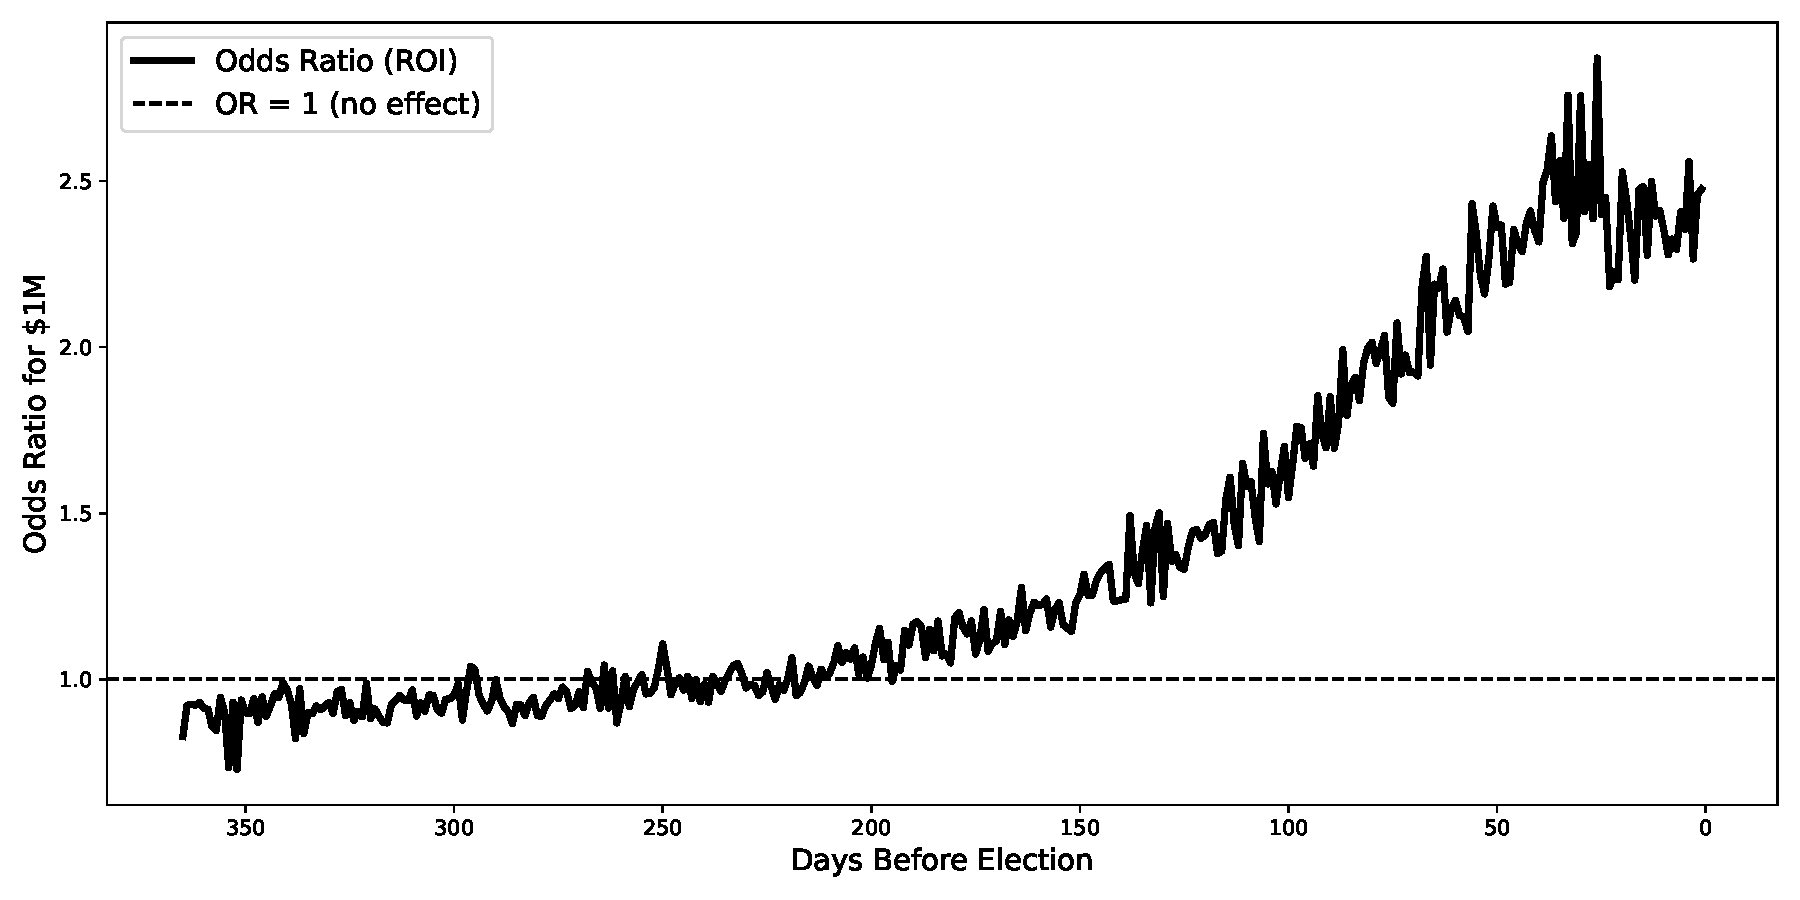
\includegraphics[width = 0.8\linewidth]{../Figures/roi_over_time.pdf}
	\caption{Total Return on Investment Trend over One Year Before Election Day}
	\label{fig:roi-year}
\end{figure}

Additional tables and plots regarding AUC, accuracy, recall, receiver operating characteristic (ROC) curves, and the raw estimated ROI $\beta$ (before converting to an interpretable odds-ratio) are collected in Appendix C.

\subsection*{6.2 Logistic GAM: Win Probability}

Table~\ref{tab:gam-log-roi} summarizes the total ROI estimates for each cutoff $X$ using logistic generalized additive models, and Table~\ref{tab:gam-log-type-roi} shows the by-type ROI estimates in the same manner (\texttt{model\_logisticGAM}). 

\begin{table}[H]
	\centering
	\begin{tabular}{||c c c||}
\hline
Days & Total ROI $\beta$ & Odds-Ratio \\
\hline\hline
360 & -0.285 & 0.752 \\
240 & 0.072 & 1.075 \\
120 & 0.198 & 1.219 \\
60 & -0.107 & 0.898 \\
30 & 0.371 & 1.450 \\
14 & 0.033 & 1.034 \\
7 & 0.308 & 1.360 \\
1 & 0.144 & 1.154 \\
\hline
\end{tabular}

	\caption{GAM Logistic Regression Total ROI Estimates}
	\label{tab:gam-log-roi}
\end{table}

\begin{table}[ht]
	\centering
	\begin{tabular}{||c c c c c c c ||}
\hline
Days & Ind $\beta$ & Ind OR & Comm $\beta$ & Comm OR & Corp $\beta$ & Corp OR \\
\hline\hline
360 & -0.037 & 0.964 & -0.399 & 0.671 & -0.529 & 0.589 \\
240 & 0.471 & 1.602 & -0.111 & 0.895 & -0.275 & 0.759 \\
120 & 0.221 & 1.247 & 0.228 & 1.257 & 0.140 & 1.150 \\
60 & -0.737 & 0.479 & 0.699 & 2.012 & -0.119 & 0.888 \\
30 & 0.039 & 1.040 & 0.320 & 1.377 & 0.868 & 2.382 \\
14 & -0.065 & 0.937 & -0.252 & 0.777 & 0.580 & 1.786 \\
7 & 0.134 & 1.143 & -0.129 & 0.879 & 1.210 & 3.353 \\
1 & 0.058 & 1.060 & -0.445 & 0.641 & 1.178 & 3.249 \\
\hline
\end{tabular}

	\caption{GAM Logistic Regression By-Type ROI Estimates}
	\label{tab:gam-log-type-roi}
\end{table}

Additional metrics, a plot of the ROC curves under this model, and a 365 day trend of the ROI are collected in Appendix C. 

\subsection*{6.3 OLS Regression: Vote Share}

In Table~\ref{tab:lin-roi}, I have collected two ways of expressing estimates of ROI based on least-squares estimates focusing on \$1 million increases in fundraising, the first being the total ROI $\beta$ (the approximation of the change in vote-share percentage points (pp) on the log-scale of dollars), and the latter being the actual marginal effect on vote share (\texttt{model\_linear.py}).

\begin{table}[!t]
	\centering
	\begin{tabular}{||c c c||}
\hline
Days & Total ROI $\beta$ & $\Delta$ \\
\hline\hline
360 & -39.8554 & -8.7519 \\
240 & -22.7274 & -4.9645 \\
120 & -3.1081 & -0.4435 \\
60 & 1.9142 & 0.5872 \\
30 & 5.7872 & 0.8855 \\
14 & 6.0042 & 0.6739 \\
7 & 5.3512 & 0.5154 \\
1 & 6.3002 & 0.6224 \\
\hline
\end{tabular}

	\caption{Linear Regression Raw and Direct ROI}
	\label{tab:lin-roi}
\end{table}

Figure~\ref{fig:feat-importance} depicts the feature importance paths --- absolute standardized coefficents --- for key predictors across cutoffs, while Figure~\ref{fig:heatmap} depicts the heatmap of least-squares $p$-values for selected predictors:

\begin{figure}[H]
	\centering
	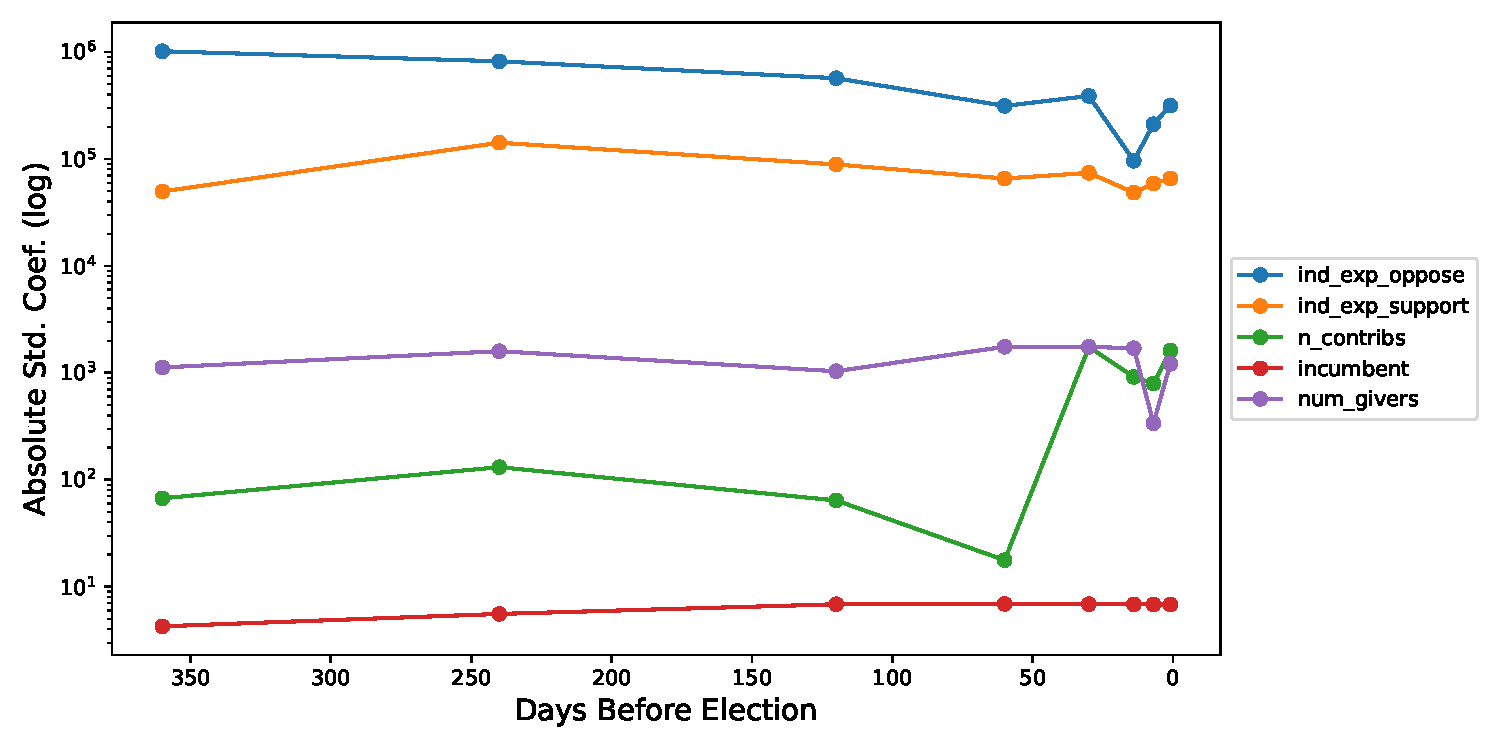
\includegraphics[width = 0.8\linewidth]{../Figures/feat_imp.pdf}
	\caption{Feature Importance Paths across Cutoffs, Logarithmic Scale}
	\label{fig:feat-importance}
\end{figure}

\begin{figure}[H]
	\centering
	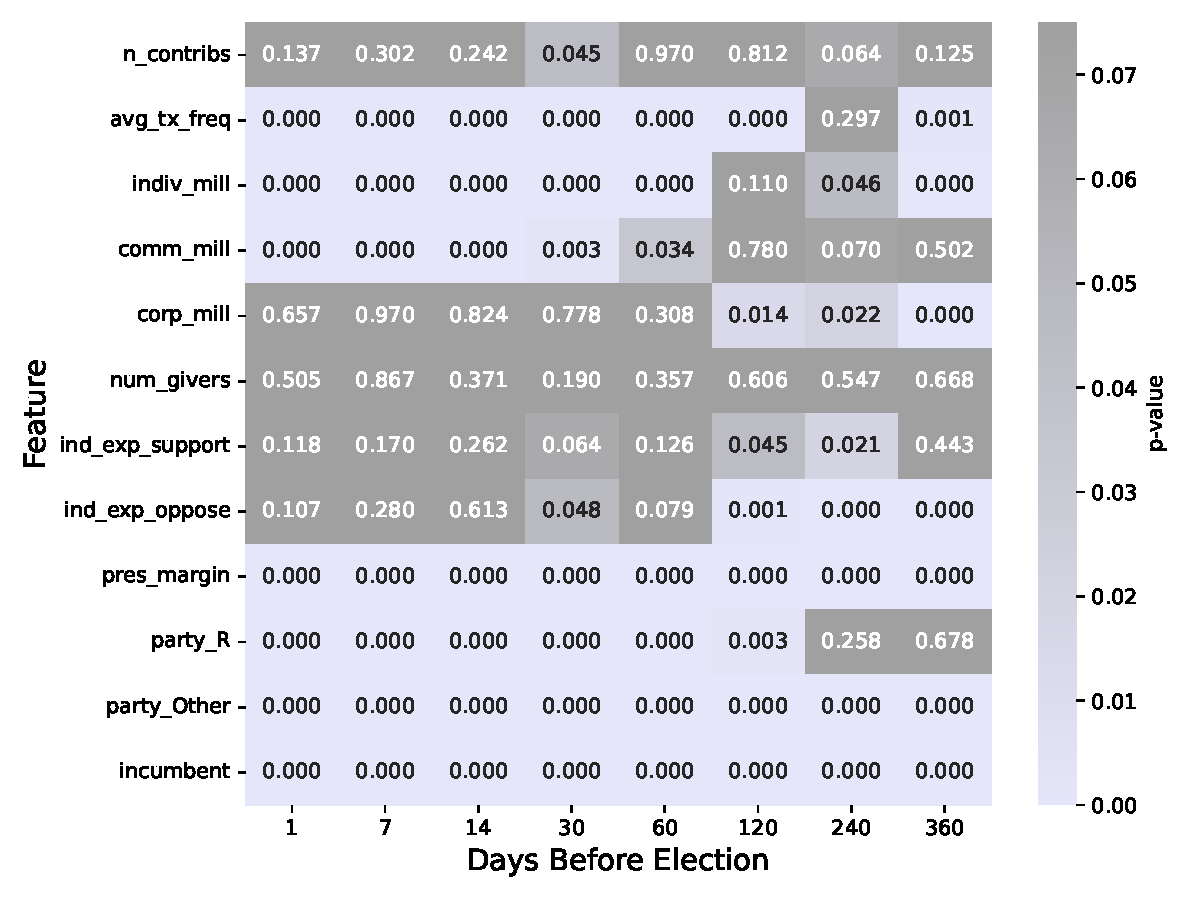
\includegraphics[width = 0.8\linewidth]{../Figures/sig_heatmap.pdf}
	\caption{Least-Squares $p$-value Heatmap for Key Predictors across Cutoffs}
	\label{fig:heatmap}
\end{figure}

Additional information concerning out-of-sample performance metrics ($R^2$, RMSE, MAE), 5-fold CV $R^2$, and regularized $R^2$, and the $\alpha$ used given the better regularization technique (Ridge or LASSO) are collected in Appendix C. 

\subsection*{6.4 Linear GAM: Vote Share}

In Table~\ref{tab:gam-lin-metrics}, I collect the repeated-$k$-fold CV metrics, as well as the GAM ROI-$\Delta$ vote-share (pp) per \$1 million total at the sample-mean mix (\texttt{model\_linearGAM.py}).

\begin{table}[H]
	\centering
	\begin{tabular}{||c c c c c||}
\hline
Days & CV $R^2$ & CV RMSE & CV MAE & $\Delta$ (pp per $1M$) \\
\hline\hline
360 & 0.488 & 12.973 & 8.523 & -1.602 \\
240 & 0.538 & 13.336 & 8.970 & -0.460 \\
120 & 0.502 & 14.837 & 9.377 & 1.741 \\
60 & 0.599 & 13.742 & 9.214 & 2.169 \\
30 & 0.659 & 12.855 & 8.817 & 0.929 \\
14 & 0.680 & 12.514 & 8.693 & -0.193 \\
7 & 0.681 & 12.527 & 8.716 & -0.278 \\
1 & 0.692 & 12.318 & 8.670 & -0.230 \\
\hline
\end{tabular}

	\caption{Linear GAM Cross-Validated Performance by Cutoff}
	\label{tab:gam-lin-metrics}
\end{table}

A supplemental table detailing the hold-out performance at each cutoff is collected in Appendix C.

\section*{7 Interpretation}

Although there is a vast amount to unpack from the results of the previous section, the models generated tell a consistent story: late-cycle fundraising, particularly from individual donors, is what really moves the needle on both probability of winning and vote-share in U.S.\ House elections. 

\subsection*{7.1 Logistic Regression}

Area under the curve rises from 0.898 at 360 days before the election to a peak of 0.942 by the day before the election. Across all specified cutoffs, accuracy is stable, ranging from 86.5 percent to 89.9 percent. Recall for class 1 (winners) ranges from 84.5 percent to 91.7 percent, while recall for class 0 (losers) ranges from 80.1 percent to 94.3 percent. Although early-cycle fundraising offers strong predictive power, substantially more signal arrives within the final two months of the campaign (see Figure~\ref{fig:roi-year}). These results are consistent with Jacobson (1978), who showed that late contributions are far more informative about eventual electoral outcomes than early money.

\indent At 360 days, the aggregate ROI odds-ratio equals 0.902, suggesting a negative association between dollars raised that early and winning --- potentially reflecting that underfunded candidates (generally challengers) raise money early but still lose; early-cycle fundraising may be more diagnostic than causal, revealing candidate quality and perceived competitiveness. In fact, Adam Bonica examined the relationship between early fundraising and electoral success, stating that ``focusing on general election contests understates the true effect of fundraising on election outcomes'' \cite{bonica2016}. Bonica found that early fundraising strongly predicted who would win primary races, but did not necessarily predict general election success.

\indent Alternatively, early fundraising may reflect not only candidate quality but also strategic front-loading by well-known incumbents to finance long-lead advertising. In other words, well-funded incumbents may raise early to buy TV in advance, so their ROI looks attenuated simply because they are shifting ``spending time'' rather than ``spending amount.'' When observing the proportion of winners versus losers across time (as shown in Section 8), the number of winners who receive donations/begin spending about a year before Election Day greatly exceeds the number of losers who do the same.

\indent According to Figure~\ref{fig:roi-year}, once one reaches 200 days before the election, ROI becomes positive up through Election Day. This is supported by the individual cutoff results, showing that, while there is variation regarding how much a \$1 million increase in receipts multiplies the odds of winning by, there are benefits to receiving donations late in the game. Stratmann (2005) argued that campaign spending has diminishing marginal returns, but those returns are highly time-sensitive, with late spending far more valuable, as validated by my results.

\indent Observing individual contributions, the ROI odds-ratio grows steadily from 1.07 at 360 days to 1.76 at seven days before leveling off at 1.69 at one day. Alternatively, the ROI of non-connected committee contributions is generally negative or near zero throughout, suggesting that this money is less effective, especially one to two weeks before the election. Another way to interpret this is that non-corporate committees tend to finance targeted voter-contact operations, which have slower lead times, and the payoff may not materialize until very late. Finally, corporate committee ROI is strongly negative at 360 days, but turns positive by 120 days, and remains high as Election Day gets closer. Therefore, it seems connected-committee spending is important for candidates, but not too early on. Individual donations are often a reflection of voter enthusiasm, whereas corporate PAC money may buy less targeted ads and thus have a weaker return on investment. 

\subsection*{7.2 GAM Logistic Models}

Compared to the simple logistic models at each cutoff, GAM-based models yielded a higher AUC overall, indicating non-linearities improve classification. ROI patterns are qualitatively similar, but quantitatively different; although the previous models showed a consistent rise in ROI estimates moving closer to the election day, the GAM model captures non-monotonic effects at later cutoffs (60 and 14 days), reflecting that at certain points diminishing returns exist. As mentioned, this is supported by a variety of research.

When observing Figure~\ref{fig:gam-or}, the dips and spikes in ROI become much more apparent. There are a few explanations as to this volatility. In a presidential-election year, the general election falls on the Tuesday after the First Monday in November. Sixty days before that, around early September, two notable things happen. First, the 60-day ``Electioneering Communications'' window opens: under the Bipartisan Campaign Reform Act (BCRA), any broadcast, cable, or satellite ad that (a) refers to a clearly identified federal candidate and (b) is publicly distributed within 60 days of a general election is defined as an ``electioneering communication'' \cite{fec_communications}. From that point forward, corporations and labor unions are prohibited from funding those ads with their general-treasury funds, and any such ad must be reported to the FEC (with details on who paid for it and how much it cost) \cite{congress_plaw}. Around the same time, both the House and Senate typically conclude their August session and return home to campaign and meet constituents. This ``recess'' gives incumbents an official break from Capitol Hill to focus on outreach back in their districts. It also often markets the start of high-profile campaign events that lead into the final two months of the cycle \cite{schedule}. So, about two months before Election Day, one sees both the formal onset of the FEC's electioneering communications restrictions/reporting requirements and Congress's late-summer recess, which ushers in the final sprint of district-and-state campaigning.

This provides a clear explanation for the odds-ratio estimate produced by the logistic GAM 60 days before the election. While two weeks before the election yields a smaller odds-ratio (1.03) compared to two weeks prior and a week after, it is still positive; however, at 60 days, there is a negative return on investment (with an odds-ratio of 0.9). This differs somewhat from the non-GAM logistic model evaluated previously, where the odds-ratio stayed relatively high within the last two months of the election, even if there was some variation.

One could also hypothesis tactical campaign pauses (major debates, party conventions, and so forth) that temporarily crowd out small-donor appeals, essentially creating ``valleys'' in effectiveness.

\subsection*{7.3 Linear Regression}

$R^2$ never rises past 61 percent, indicating that factors besides money, incumbency, and party-district fixed effects explain the variation in vote share. Total ROI, measured as percentage points (pp) of vote-share per \$1 million, moves from strongly negative at -8.75 pp at 360 days to a peak of 0.89 pp at 30 days, tapering off at 0.62 pp at one day. Early-cycle dollars are often picked up by candidates already weak in the polls, hence the negative coefficent. As the season progresses, fundraising increasingly captures true electoral momentum (corroborated by the binary results).

The regularization models (Ridge and LASSO) give nearly, if not exactly, identical $R^2$ but trim down erratic coefficients. These similar results suggest there is little overfitting in this training; the model's level of complexity is not significantly inflating its performance on the training set. Also, feature importances consistently rank independent expenditures against the candidate and independent expenditures in support of the candidate as top predictors --- underscoring the outsized impact of outside spending. Incumbency, party, district partisanship, average transaction type frequency, and the amount of money (in millions) given by individuals remain extremely strong predictors at each cutoff, as indicated by the feature significance across cutoffs.

\subsection*{7.4 Gam Linear Models}

Cross-validated $R^2$ is lower early but peaks at around 69 percent one day before the election, while hold-out $R^2$ peaks in the two-week window. The change in vote share per \$1 million flips from negative to positive between 240 and 120 days before the election, then becomes negative toward the very end of the election cycle, suggesting over-saturation or that last-minute money may be reactive to impending loss rather than causally effective. Once flexibly accounting for splines in all features, the very last-minute money may not further boost vote share on the linear scale --- consistent with diminishing marginal returns. 

\indent Four things stand out throughout this study: first, across every model, the predictive power and causal return on investment of campaign contributions is time-varying, with negligible or negative returns early. There is more variation as Election Day approaches, with the GAMs indicating more money does not increase one's probability of winning or vote share too close to that date. Next, individual donations steadily gain value as they signal voter enthusiam; non-corporate PAC and other committee money is at best neutral; corporate funds have a lagged but positive effect mid- to late-cycle. Third, even after adjusting for money, incumbency and district partisanship dominate. This echoes Jacobson (2004) who argued that the money-win link is conditional on the underlying political environment. Finally, GAMs reveal thresholds and saturation points that linear models do not pick up, suggesting strategic timing of fundraising appeals can yield disproportionately higher gains. Ultimately, the dynamic timing of ROI is a critical nuance that extends the classic findings of Jacobson and more recent non-linear analyses in the campaign-finance literature.

\section*{8 Limitations and Interpretation Caveats}

To start, because GAMs are nonlinear, the derivative changes with the input values. Consequently, by computing finite differences at the mean, I capture only the average partial effect there --- an estimate that may fail to represent slopes at other points in the covariate domain. Also, all ROI $\beta$s, ORs, and elasticities reported here reflect associational effects --- ultimately, how an additional \$1 million is correlated with higher win odds (or vote share) in our sample, holding other covariates at their means. 

\indent A clear class imbalance exists when predicting winners versus losers across some cutoffs; for example, at $360$ days before the election, proportionally, about 80 percent of the data consists of winners. Intuitively, this makes sense: as Election Day approaches, there is more of a 50:50 split between winners and losers, but earlier on, not everyone has received contributions. The AUC is however still high for each model across each chosen cutoff. Similarly, the recalls for class 1 (winners) and class 0 (losers) are relatively high, with the lowest recall value being for class 0 at 360 days of 0.724. Although the GAMs performed better in terms of AUC, accuracy, and class 1 recall, they performed worse in terms of class 0 recall, indicating that predictive accuracy of the minority class was worse under the generalized additive model. The difference is not drastic, but it is something to note: this is simply a result of how the fundraising process goes.

\indent When observing the odds-ratio trend across a 365 day period for the logistic model, a more-or-less upward trend is apparent. Furthermore, Figure~\ref{fig:gam-or} depicts how the logistic GAM's ROI fluctuate over time. Note, however, the numbers generated for each ROI $\beta$ (across \textit{all} models) in the study are based on arbitrary cutoffs for snapshot comparisons. Although overall trends are implied (and validated by existing literature), there may be greater variation across time than what is seen solely from the eight cutoff days examined. Different or more granular cutoffs might reveal subtler temporal patterns.

\indent A drastic dip occurred in the hold-out $R^2$ at 120 days for the linear GAM, signaling perhaps potential under- or over-smoothing for that slice of data, meaning additional tuning may be necessary to achieve improved results.

\indent $R^2$, for this project, only serves to tell us the percentage of variation in vote share that may be explained by the features within the models. The lower $R^2$s obtained within this project do not automatically disqualify these models as bad or inaccurate nor the estimates as useless. Even with low $R^2$s, one may still draw important conclusions about the relationships between variables, particularly if the independent variables are statistically significant (see Figure~\ref{fig:heatmap}).

\section*{IX Conclusion}

In this paper, I offer a comprehensive, multi‑model assessment of how the timing of U.S.\ House campaign contributions affects marginal win probabilities and vote share. By comparing four modeling approaches --- logistic regression, logistic GAMs, least-squares, and linear GAMs —-- across eight pre‑election snapshots, I have shown the following:

\begin{enumerate}
	\item \textbf{Early‐cycle contributions} ($\geq$ 240 days out) exhibit negligible or even negative marg\-inal associations with both win probability and vote share, likely reflecting the confounding influence of candidate quality and district partisanship.
	\item \textbf{Mid‐ to late‐cycle contributions} (120–14 days out) yield the strongest positive returns, with individual donations outperforming committee funds. 
	\item \textbf{Very last‐minute spending} (seven to one days out) continues to boost win odds on the logit scale but shows signs of saturation on the linear vote‑share scale, consistent with diminishing marginal returns.
	\item \textbf{GAMs uncover non-monotonic patterns} that linear models miss —-- namely local dips and plateaus in ROI, highlighting the strategic value of timing in campaign finance. 
\end{enumerate}

These findings offer actionable benchmarks for donors who must allocate finite resources across the calendar. More broadly, they underscore that the effectiveness of campaign spending is both \emph{time‑sensitive} and \emph{context‑dependent}, in line with theoretical expectations from political–economy and persuasion models.

In light of this, consider the following example. A donor must decide how to allocate a finite advertising budget over the course of the pre-election period, aiming to maximize the probability of his or her chosen candidate's victory in a congressional race. Contributions can be made on any day before the election, but their effectiveness varies by timing, as estimated from historical data using any of the above models. Let $t \in \{1,2, \cdots, 365 \}$ index the days before the election, and the decision variable $b_t$ represent the amount of spending allocated on day $t$. To maximize the candidate's predicted win probability, given a logistic model:

\[ \underset{\{b_t \geq 0 \}}{\max} \Lambda^{-1} \Big[ \alpha + \sum\limits_t \beta_t \log(1 + b_t) \Big] \]

\noindent where $\Lambda(\cdot)$ is the logistic function and $\beta_t$ is the empirically estimated ROI coefficient for spending on day $t$, obtained from (for this example) the GAM logistic model. $\alpha$ captures the baseline win odds given other control effects, such as incumbency, political party, etc. The budget constraint is naturally expressed as $\sum\limits_t b_t \leq B$, where $B$ is the total available budget, and this spending must be non-negative for all $t$. 

Having estimated the ROI coefficients for each day ($t = 1, \ldots, 365$) using the logit GAM, a donor should allocate her budget proportionally to those coefficients (as a higher return on investment means a higher marginal benefit). Solving the full nonlinear optimization problem, where the win probability is the logistic function shown above, reveals the optimal spend for each cutoff day. The first-order condition suggests spending should equalize the marginal contribution to the log-odds of victory across days, adjusted for diminishing returns:


\[ \dfrac{\partial}{\partial b_t} \Lambda^{-1} \Big[ \cdots \Big] \propto \dfrac{\beta_t}{1 + b_t} \]

From this, a higher $\beta_t$ (higher ROI) and lower $b_t$ (less spending in period $t$ before adding an additional dollar) will favor more allocation to that time period. Considering the ROI $\beta$s for this model are constants over the $365$ day period, changing the budget and $\alpha$ parameter will not change which days are most beneficial to spend on, but they do change, respectively, how much should be allocated each day and the maximum probability of winning a candidate will experience (given the baseline probability he or she is starting with). Ultimately, coinciding with Figure~\ref{fig:gam-or}, a donor should focus largest spends approximately three to six weeks before Election Day; earlier and much later spending is less efficient per these ROI estimates. Under uncertainty, a robust allocation (using a lower-bound $\beta_t$) would further favor that same window, but more conservatively. 

Now, throughout this paper, I have documented how campaign contributions to U.S.\ House candidates accumulate over time and how relative fundraising advantages appear to correlate with electoral outcomes. To deepen our theoretical understanding of these patterns, one can recase the fundraising ``race'' as a two-player strategic contest. Below, I outline the key ingredients of such a model:

Consider two players: candidate A's campaign (the incumbent or challenger on one side) and candidate B's campaign (the opposing side). Each campaign acts as a profit-maximizing agent seeking to maximize its net expected payoff from victory minus fundraising costs.

Campaigns choose how much to raise (and equivalently to spend) over the pre-election horizon. Two formulations are common:

\begin{enumerate}
	\item Static (one-shot) model --- Each player selects a total fundraising level
		\[ b_i \geq 0, \hspace{1em} i \in \{A, B\}, \]
		representing all contributions collected by election day.
	\item Dynamic (multi-period) model --- The horizon is divided into $T$ discrete time windows (for example, 360 days, 240 days, $\ldots$, 1 day before Election Day). In each period $t$, campaign $i$ chooses
		\[ b_{i,t} \geq 0, \]
		subject to an overall fundraising budget
		\[ \sum\limits_{t=1}^T b_{i,t} \leq B_i. \]
\end{enumerate}

\noindent In both cases, $\mathbf{b}_i$ (or $b_i$) is publicly observed by the opponent (or inferred through disclosure).

The probability that A wins the election is modeled as a monotonic function of the two sides' ``effort'' (funds raised). A standard choice is the Tullock contest success function (CSF), a simple and widely used way to model how players' ``efforts'' (or expenditures) translate into their probability of winning a contest or obtaining a prize \cite{tullock1980}. Introduced by Gordon Tullock, the Tullock CSF is often applied in the context of rent-seeking, but it also easily maps spending into probabilities of winning seats in political competition:

\[ p_A (b_A, b_B) = \dfrac{b_A^\alpha}{b_A^\alpha + b_B^\alpha}, \hspace{1em} p_B = 1 - p_A, \]

\noindent where $\alpha > 0$ captures effectiveness of funds ($\alpha = 1$ is proportional effect, $\alpha < 1$ exhibits diminishing returns, and $\alpha > 1$ exhibits increasing returns). In a dynamic model, one can define an \textit{interim} CSF after period t: 

\[ p_{A,t} = \dfrac{\Bigg(\sum\limits_{s=1}^t b_{A,s} \Bigg)^\alpha}{\Bigg(\sum\limits_{s=1}^t b_{A,s} \Bigg)^\alpha + \Bigg(\sum\limits_{s=1}^t b_{B_,s} \Bigg)^\alpha}, \]

\noindent with $p_{A,T}$ as the final win probability.

Each player weights the value of winning against the cost of raising funds. For campaign $i \in \{A, B \}$, denote by $V_i =$ the value of winning the seat (could differ by incumbency, seat prestige, and so forth) and by $c_i (b) =$ the cost of raising $b$ dollars where $c_i^{''} (b) > 0$, that is, $c(\cdot)$ is convex.

\noindent Then the static payoff is

\[ U_i (b_i, b_j) = p_i (b_i, b_j) V_i - c_i (b_i). \]

\noindent In the dynamic setting, one can write

\[ U_i ( \{b_{i,t} \}, \{b_{j,t} \}) = p_{i,T} V_i - \sum\limits_{t=1}^T c_i (b_{i,t}). \]

Commonly, $c_i (b) = k_i b + \dfrac{1}{2} \lambda_i b^2$, with $k_i, \lambda_i > 0$, so that raising additional dollars becomes progressively more expensive.

A pure-strategy, Nash equilibrium consists of fundraising decisions for all campaigns where no single campaign can gain by unilaterally altering its decision:

\[ b_i^* = \text{arg} \underset{b_i \geq 0}{\max} \Big\{ p_i (b_i, b_j^*) V_i - c_i (b_i) \Big\}, \hspace{1em} i \in \{A, B \}. \]

Under $\alpha > 0$ and strictly convex cost functions $c_i$, the best response curves cross exactly once, yielding a unique interior Nash equilibrium \cite{bayes}. Closed-form solutions arise in special cases (for example, linear costs, $\alpha = 1$):

\[ b_i^* = \dfrac{V_i}{2 \lambda_i} - \dfrac{k_i}{2 \lambda_i} + \text{terms depending on } V_j, k_j, \lambda_j. \]

\noindent Once ($b_A^*, b_B^*$) is characterized, one can derive the following:

\begin{enumerate}
	\item A larger $V_i$ implies  more aggressive fundraising.
	\item The higher is $\alpha$ the greater are the returns to additional dollars.
	\item The higher the marginal cost the lower are fund-raising levels.
	\item Asymmetries (incumbency, baseline name recognition) can be modeled via a ``starter-kit'' endowment $b_{i,0} > 0$.
\end{enumerate}

These comparative static results illustrate, for example, why open-seat contests or expensive districts see more extreme fundraising arms races. To capture the temporal profile of fundraising (as in my cutoff analysis at 360 days, 240 days, and so forth), the model extends naturally to a $T$-period game:

\begin{enumerate}
	\item Simultaneous moves: At each $t = 1, \cdots, T$, campaigns choose $b_{i,t}$.
	\item Cumulative CSF: Interim win probability updates each period.
	\item Budget constraint: $\sum\limits_{t=1}^T b_{i,t} \leq B_i$.
	\item Solution method: Either open-loop control (treating the full vector $\{b_{i,t} \}$ as decision variables) or closed-loop (dynamic programming with state variables $\sum\limits_{s=1}^{t-1} b_{i,s}$).
\end{enumerate}

Optimal paths $\{b_{i,t}^* \}$ can reveal, for instance, whether it is optimal to front-load spend early to ``lock in'' momentum or to reserve funds for a final surge.

I have intentionally kept this framework abstract so that future researchers can estimate $\alpha$ and cost-function parameters using DIME data and election outcomes; numerical root-finding or equilibrium-solving routines may be utilized (should closed-form fail for complex cost structures); the multi-period game may be solved via dynamic programming or optimal control techniques; and stochastic shocks (for example, major outside fundraising events), informational asymmetries (private signal models), or multiple donor types (fractional contributions) may be incorporated in as robustness extensions. Such empirical and computational steps lie outside the scope of the present paper but represent a rich avenue for deepening our understanding of competitive fundraising dynamics. By embedding the fundraising context in this game-theoretic scaffold, I both clarify the strategic logic behind observed contribution trajectories and lay out a roadmap for rigorous estimation and simulation in future studies.

Naturally, some limitations associated with the above game-theoretic model exist. To start, in practice, FEC disclosures lag and contributions arrive in lumps. This can undermine the open-loop versus closed-loop solution concept --- if a campaign can not react in real time to the opponent's choices, the equilibrium notion should be Bayes-Nash with incomplete information, not a straightforward Nash equilibrium in each subgame.

Moreover, the dynamic payoff mentioned above treats dollars raised equally across all $t$. Yet, in reality, money raised early covers longer ad buys and carries opportunity costs differently than last-minute cash. A discount factor on future payoffs or costs could be introduced, or $c_i$ itself could vary by $t$ to reflect media-market pricing. Continuing with the discussion of money, in many campaigns, fundraising is endogenous and uncapped \textit{ex ante}, with the cost function serving as the only brake. Imposing an exogenous ``budget'' may be motivated by donation fatigue, donor limits, or internal campaign targets, but the ``budget'' constraint, though simplifying the problem, is not necessarily realistic.


In conclusion, by quantifying time-varying ROI and embedding it in a clear decision framework, campaigns may determine not just what matters (that is, finances, incumbency, party-district fixed effects, and so forth), but also at what points in time and how much to spend for maximal impact. 

\newpage

\section*{Appendices}

\subsection*{Appendix A}

All code, demonstrating the filtering, cleaning, adjusting for inflation, aggregation, and modeling, are documented here for full reproducibility.

\subsubsection*{\tt dime\_filtered.py}

As mentioned, the database being utilized in this script is the dime\_v4.sqlite3 database, found at the Database on Ideology, Money in Politics, and Elections website through Stanford University. Throughout this project, I intended to only utilize data on U.S.\ House elections. Therefore, in this initial script, I filtered the data based on this restriction and placed it in a new database for efficiency and space.

I began by importing the necessary packages --- the most important being {\tt duckdb} --- and then connecting to the new database I wanted to fill ({\tt dime\_house.duckdb}). Three tables existed within the original database: {\tt candDB}, {\tt contribDB}, and {\tt donorDB}. The first I filtered using three variable requirements; I specified that {\tt seat} should equal {\tt federal:house}, {\tt cycle} (which was cast as an integer) should lie between the years 2000 and 2024, and {\tt bonica\_rid} (the unique identifier for a contribution recipient) should not be null. I placed all these observations within a new table {\tt candDB\_house}.

To ensure I obtained the relevant observations from the other tables, I collected distinct {\tt bonica\_rid}s from {\tt candDB\_house} and placed these in a temporary table {\tt house\_rids}. From there, it was straightforward to filter {\tt contribDB} into {\tt contribDB\_house}; from {\tt contribDB}, I selected the observations where {\tt bonica\_rid} fell within {\tt house\_rids}, {\tt seat} was equal to {\tt federal:house}, and {\tt date} (which was cast as a date) fell between January 1, 1998 and December 31, 2024.

The {\tt bonica\_cid}s are a unique contributor ID for the candidate, allowing one to join the {\tt contribDB} and {\tt donorDB} tables. Thus, I also extracted the unique {\tt bonica\_cid}s from the {\tt contribDB\_house} and placed them in a temporary table. With this, I was able to filter {\tt donorDB} into {\tt donorDB\_house} by collecting observations with the {\tt bonica\_cid}s contained in the temporary table. 

Everything in this process was saved to {\tt dime\_house.duckdb}.\footnote{Since it became obsolete (for my purposes) once the final database was created, and it is quite a large file, this database is only available upon request.}

\subsubsection*{\tt cleaning\_by\_variables.py}

In this file, I connected to a new database {\tt dime\_house\_clean.duckdb}. To understand what variables were important for my project, I needed to observe the variables within each table.

Starting with the candidate table, I found that the majority of variables simply introduced clutter; many were identifiers, metadata, redundant, or advanced ideological scores that were unrelated to my analysis. Identifiers/names are not predictors of votes, and NIMSP (National Institute for Money in State Politics) features come from state-level sources. Ideological scores, though interesting, will not affect a candidate's probability of winning, and the metadata included in {\tt candDB\_house} was not useful for me. I kept the variables specified in Section 4 and dropped all others within {\tt candDB\_house}. 

Next, I examined the contributions table, where most variables were descriptive (last name, first name, occupation, and so forth). Geographic (such as longitude and latitude) and financial (such as memos and transaction IDs) features were included, but those were unnecessary for my analysis. Therefore, I only kept the nine variables I described in Section 4 and dropped all others within {\tt contribDB\_house}.

Finally, I explored the donor/contributor table. All variables here were either related to specific donors or already contained in one of the previous tables. Because I found none of these variables relevant for my use, I dropped the entired table {\tt donorDB\_house}.

\subsubsection*{\tt cleaning\_nulls.py}

Having filtered for the most important observations and variables, I next worked with the {\tt dime\_house\_clean.duckdb} database, cleaning the data further. For both the candidate and contributions table, I explored the types of each variable and the number of unique values.

Before proceeding with the cleaning process, I joined both tables on their matching values. {\tt candDB\_house} contained about 23,379 rows while {\tt contribDB\_house} contained about 98 million rows. Naturally, the joined table {\tt house\_joined} consisted of approximately 98 million observations. 

To bring down the amount of data I worked with, I observed the null count within each column. However, just because a value is null does not necessarily mean it should be removed; I took care with what I eliminated. Unsurprisingly, {\tt election\_type} defines the election type (general, primary, and so on). From here, I decided to work only with general elections, removing all else. Moreover, 13,933,493 observations remained after removing the null values within this column.

Next, I focused on my dependent variables {\tt gwinner} and {\tt gen\_vote\_pct}; getting rid of those nulls left me with 9,447,843 rows. The number of {\tt transaction\_type}, {\tt district\_pres\_vs}, and {\tt contributor\_type} nulls were all relatively small, leaving me with 9,430,440 observations. Finally, the null {\tt is\_corp} values were representative of whether or not a committee was a corporate entity or q trade organization. Eliminating these observations would have rendered this variable meaningless; thus, I converted all null values to 0 and the value {\tt corp} to 1.

\subsubsection*{\tt conversion.py}

In this script, I created my final database {\tt dime\_house\_clean.duckdb}, converting everything to numeric values to that they could be utilized in the modeling processes.

To start, I adjusted for inflation. Using Consumer Price Index data from the Bureau of Labor Statistics, I created a table containing CPI-based deflators with 2024 as the base year. By joining the deflator table {\tt deflator\_to\_2024} on to house table and multiplying every dollar column by {\tt deflator\_to\_2024}, all monetary variables were converted to 2024 dollars.

Next, I computed a new variable {\tt days\_before}, representing the number of days before an election that a contribution was given. Considering general elections typically fall on the first Tuesday after the first Monday in November, I ``found'' this date for each election cycle and calculated how many days fell between Election Day and the day one donated funds.

With this, I removed/encoded/transformed the remaining columns. Because I only worked with general elections, {\tt election\_type} was dropped. Original monetary value columns were dropped due to deflation, and {\tt date} was dropped due to {\tt days\_before}. {\tt district} was also dropped; while district-level heterogeneity is important to capture, the district variable itself introduces too much cardinality to be useful. Alternatively, Jacobson used a continuous partisanship measure to control for how Democratic or Republican a district is without needing over 400 dummy columns. Similarly, I retained {\tt district\_pres\_vs} to account for this.  

{\tt contributor\_type} measures whether the contributor was an individual versus a committee/organization, so I mapped individual to 0 and all else to 1. {\tt ico\_status} was transformed using one-hot encoding. {\tt transaction\_type} would have resulted in 51 dummy variables, so I utilized frequency encoding to reduce this. Lastly, for {\tt gwinner}, measuring whether a candidate won or lost, I converted winning observations to 1 and losing observations to 0.

The raw {\tt transaction\_type} column and deflator column were both removed, resulting in a {\tt house} table ready for aggregation and modeling.

\subsubsection*{\tt aggregation.py}

In this script, I connected to the pre-cleaned database {\tt dime\_house\_cleaner.duckdb} containing the {\tt house} table. As described in Section 5, I defined a set of ``cutoffs'' (look-back periods) in days before Election Day.

For each cutoff, I sliced the data to only include contributions made up to that point. Next, I aggregated summary statistics per candidate $\times$ cycle, including counts, average frequencies, sums of dollars by source, campaign totals, party and outcome flags. The resulting aggregations were written to Parquet files for fast downstream loading and reproducibility.

This script involves a time-series of fundrasing ``snapshots'' at multiple pre-election milestones --- ideal for modeling how fundraising patterns relate to electoral outcomes. 

\subsubsection*{\tt model\_logistic.py}

I begin by importing {\tt os}, {\tt numpy}, and {\tt pandas}, along with {\tt scikit-learn} modules for logistic regression, model evaluation, data splitting, scaling, and pipelines, as well as {\tt Matplotlib} for plotting. Then, I pull the data from the previously generated Parquet files and re-use the same list of cutoff days that define how far in advance of each election the fundraising snapshot was taken. Before diving into the loop, I prepared empty Python lists to collect performance metrics, regression coefficients, per-type derivatives, and elasticities. I also initialized a figure for overlaying multiple ROC curves.

Inside the loop, for each cutoff $X$ (where $X \in \{360, 240, 120, 60, 30, 14, 7, 1 \}$), I read the corresponding Parquet file into a DataFrame, selected a handful of features --- transaction counts and frequencies, logged money variables (individual, committee, and corporate contributions), plus campaign covariates like number of givers, independent expenditure support/opposition, presidential margin, and party/incumbency flags --- and designated the binary {\tt won\_general} as the target. The three money features were log-transformed via {\tt np.log1p} to stabilize their distribution. Data was split 75:25 into training and testing sets with stratification on the outcome. A pipeline standardized the features and fit an L2-penalized logistic regression (with a large $C$ to approximate unpenalized estimates) using the {\tt lbfgs} solver.

Once trained, the model predicted both class labels and probabilities on the test set. I computed and printed the ROC AUC, overall accuracy, recalls for both positive and negative classes, the full confusion matrix, and a classification report. I then extracted the three coefficients on the logged money features from the fitted model, summed them to get a ``total ROI $\beta$,'' and printed both the $\beta$ and its odds ratio ($exp \beta$), as well as the individual $\beta$ and OR for each money type. To translate this into an economic interpretation, I calculated a point-estimate elasticity by multiplying the total $\beta$ by the ratio of average fundraising to average win probability. That elasticity was then printed and stored. Meanwhile, I added the ROC curve for this cutoff to the common plot, labeling each curve with its AUC.

After cycling through all cutoffs, the plot was finalized and saved as a PDF. Finally, I constructed five summary tables as pandas DataFrames (performance metrics, total ROI $\beta$ and OR, per-type ROI $\beta$ and OR, raw elasticities, and normalized elasticities), writing each to LaTeX files.

\subsubsection*{\tt model\_logisticGAM.py}

The workflow in this script parallels the pure-logistic script but replaces the linear model with a semiparametric generalized additive model to capture potential nonlinearities in how campaign features predict electoral sucess. After importing necessary libraries --- including {\tt pygam} for GAMs, {\tt sklearn} utilities for data handling and metrics, and {\tt Matplotlib} for plotting --- I use the same list of cutoffs and Parquet files utilized before. Empty Python lists were initialized to store AUCs, accuracies, recalls, ROI coefficients, per-type derivatives, baseline probabilities, and elasticities, and a figure was prepared for superimposing ROC curves.

For each cutoff $X$, I read in the appropriate files, logged the three fundraising variables with {\tt log1p}, and assembled a feature matrix splitting continuous covariates (transaction counts/frequencies, the logged money variables, number of givers, independent expenditure support/opposition, presidential margin) from categorical flags. Everything was standardized via a {\tt StandardScaler}, then randomly stratified into training and test sets. GAM terms were constructed by combining ten-knots spline terms for each continuous feature and factor terms for each categorical indicator; I fit the resulting model using a coarse grid search for smoothness parameters with up to 10,000 iterations.

Once trained, probabilities and class predictions on the test data yielded standard metrics --- AUC, accuracy, recall for both classes, a confusion matrix, and a classification report --- which were printed and stored. To quantify a ROI analog, I computed finite-difference derivatives of the predicted win probability with respect to each logged money variable, evaluated at the mean feature vector. I averaged these partial effects (weighted by each money type's share of average fundraising) to obtain an overall change in win probability per unit dollar change; transforming this via the logistic link function resulted in a total ROI $\beta$ (with its odd ratio), and each component $\beta$ was similarly derived. I then computed elasticity by scaling the total $\beta$ by the ratio of mean fundraising to mean win probabilities. All these values were printed and appended to lists. Just as before, I overlaid on an ongoing plot the ROC curve for each cutoff.

Finally, I collated the results into five LaTeX tables, the same as in the MLE logistic process.

\subsubsection*{\tt model\_linear.py}

I began by importing both classical and penalized regression tools --- {\tt statsmodels} for least-squares inferences and {\tt scikit-learn}'s {\tt LinearRegression}, {\tt RidgeCV}, and {\tt LassoCV} --- alongside utilities for splitting data, scaling features, cross-validation, performance metrics, and plotting. Pointing to the same directory of Parquet snapshots at cutoffs 360, 240, 120, 60, 30, 14, 7, and 1 day(s) before each election, I initialized lists to collect elasticities, total ROI coefficients, marginal $\Delta$ per \$1M, test-set and cross-validated $R^2$, RMSE, and MAE, as well as lists specifying which regularized model wins (Ridge or LASSO), its chosen $\alpha$, and its out-of-sample $R^2$. I also prepared structures to track standardized feature importances over time for key predictors and to record least-square $p$-values for every base feature.

For each cutoff, I loaded in the appropriate Parquet file, constructed a feature matrix, log-transformed the three fundraising columns, and set the Democratic two-party vote share {\tt gen\_vote\_pct} as the continuous target. Next, I performed a 75:25 train-test split and fit a simple pipeline (standard scaler $+$ OLS) on the training data. I then printed each model's test $R^2$, RMSE, MAE, and 5-fold cross-valited $R^2$ on the full dataset. To understand statistical significance, I ran a {\tt statsmodel} ordinary least-squares model on the training set, yielding coefficient estimates, standard errors, and $p$-values; from this, I extracted and printed the top five standardized coefficients (absolute value) and stored these importances and $p$-values for later.

Following this, I computed a total ROI $\beta$ by summing the three coefficients on individual, committee, and corporate fundraising (back-transformed to ``pp per \$1M''), and printed it. I then estimated the marginal change in vote share at the average fundraising mix by slightly bumping each log-transformed column according to its share of total spend, predicting before/after vote share, and taking the difference. Elasticity involved multiplying $\beta$ by the ratio of mean fundraising to mean vote share.

To guard against overfitting and potentially improve predictive power, I retrained on the full feature set two penalized models --- RidgeCV and LassoCV --- each with a logarithmically spaced $\alpha$ grid and 5-fold cross-validation. I compared the test $R^2$s on a fresh 75:25 split; selected the stronger model; recorded its name, optimal $\alpha$, and out-of-sample $R^2$; and printed its top five standardized coefficients.

After looping through all cutoffs, I normalized and printed the elasticities to show relative importance across time. I then generated two diagnostic figures: a log-scale line plot of each tracked feature's absolute standardized coefficient versus days before the election (to visualize how predictor importance evolves), and a grayscale heatmap of least-squares $p$-values for each feature across cutoffs (highlighting statistical significance trends).

Finally, I wrote four LaTeX tables regarding ROI versus marginal $\Delta$, performance metrics, best regularized model and $R^2$, and elasticities.

\subsubsection*{\tt model\_linearGAM.py}

For the final models, I implemented a semiparametric regression to predict two-party vote share as a smooth function of campaign metrics, using GAMs. Beginning by importing standard libraries such as {\tt numpy} and {\tt pandas}, {\tt pygam} for splines and factor terms, {\tt scikit-learn} utilities for scaling and data splitting and {\tt Matplotlib} for plotting, I followed a similar process as what I did previously. After establishing the pre-election cutoffs, I initialized lists to collect cross-validation and hold-out performance metrics, finite-difference estimates of the marginal change in vote share per \$1M (``$\Delta$ pp per \$1M), and elasticities. I defined a logarithmic grid of smoothing penalties and eight spline basis functions, along with a repeated $k$-fold scheme for robust tuning.

For each cutoff $X$, I loaded the aggregated DataFrame, log-transformed the three fundraising variables, and constructed feature lists: continuous covariates and categorical indicators. After standardizing all predictors, I built a GAM formula combining spline terms for each continuous feature with factor terms for each category. Using repeated $k$-fold cross-validation, I grid-searched over the smoothing penalty grid for each fold, fit a {\tt LinearGAM}, and recorded mean and standard deviation of out-of-sample $R^2$, RMSE, and MAE across folds. I then re-fit the optimally smoothed GAM on a held-out 25 percent test split, reported its hold-out metrics, and computed finite-difference derivatives of the GAM's prediction at the mean predictor vector for each money variable. By weighting these derivatives according to each fundraising source's share of average spending, I obtained a single marginal $\Delta$ pp per \$1M and, from there, an elasticity normalized by the mean vote share.

After processing every cutoff, I wrote three LaTeX tables --- cross-validated performance plus $\Delta$, hold-out metrics, and elasticities. The result is a fully automated pipeline that delivers both nonlinear model performance diagnostics and economic-interpretation metrics for how incremental fundraising at different horizons translates into expected changes in vote share.

\subsection*{Appendix B}

This section contains descriptions of the variables utilized throughout my entire cleaning/modeling process, as well as descriptions of how those variables were transformed to meet my needs. Descriptions of the original variable names come from the DIME codebook.

\texttt{cycle}: The two-year election cycle during which the contribution was recorded. Cast as INTEGER during null cleaning process.

\texttt{bonica\_rid}: Unique ID assigned to candidates; used to join candidate table with contributions table. Decimals removed to match with \texttt{bonica\_cid}.

\texttt{bonica\_cid}: Unique contributor ID for candidate; used to join contributions table with donor table. Cast as BIGINT during null cleaning process.

\texttt{party}: Party of candidate. Converted to three dummies (representing 'Republican', 'Democrat', or 'Other') during aggregation process.

\texttt{seat}: Office sought. Only used in initial database filtering to retrieve all U.S.\ House elections.

\texttt{ico\_status}: Incumbency status. Converted to dummy variables, but only dummy used was \texttt{is\_incumbent} and renamed \texttt{incumbent}.

\texttt{num\_givers}: Number of distinct donors that gave to the candidate during a specific election cycle.

\texttt{ind\_exp\_support}: Sum total independent expenditures made to support the candidate.

\texttt{ind\_exp\_oppose}: Sum total independent expenditures made to oppose the candidate.

\texttt{gen\_vote\_pct}: FEC reported vote share in general election; continuous dependent variable in linear model and linear generalized additive model.

\texttt{gwinner}: General election outcome; binary dependent variable in logistic model and logistic generalized additive model. Encoded to numeric 1s and 0s. During aggregation process renamed \texttt{won\_general}.

\texttt{district\_pres\_vs}: District-level percentage of the two-party vote share won by the Democratic presidential nominee in the most recent (or concurrent) presidential election. During aggregation process renamed \texttt{pres\_margin}.

\texttt{contributor\_type}: Specifies whether contributor is an individual or a committee/organization. Converted to numeric, and then renamed \texttt{contrib\_type}. 

\texttt{is\_corp}: Specifies whether the contributor is a corporate entity or q trade organization (only applies to committees). NULL if contributor is neither. Converted to 1s and 0s during NULL cleaning process.

\texttt{amount}: Dollar amount of contribution.

\texttt{date}: Transaction date of contribution. Cast to DATE in NULL cleaning process. Removed after used to calculate \texttt{days\_before} variable.

\texttt{election\_type}: Specified whether the election was a primary, general, etc. Removed once database was filtered for only general elections.

\texttt{days\_before}: Number of days before an election that a contribution was received. Calculated by identifying the election date for a given cycle as the first Tuesday after the first Monday of November, then taking the difference between that date and the date a contribution was received.

\texttt{n\_contribs}: Total number of contributions. Calculated during aggregation process by summing the total amount of contributions a candidate received within a particular election cycle.

\texttt{avg\_tx\_freq}: Average transaction type frequency. Calculated using \texttt{tran\-sac\-tion\_type} variable. Initial variable was frequency-encoded during conversion process. The average was taken during the aggregation process to obtain the average transaction type frequency for each candidate in a given cycle.

\texttt{indiv\_mill}: Amount in millions that a candidate received from individual donors. Calculated by taking the proportion of the total amount given to a candidate by individuals.

\texttt{comm\_mill}: Amount in millions that a candidate received from a non-corporate committee. Calculated by taking the proportion of the total amount given to a candidate by non-corporate committees.

\texttt{corp\_mill}: Amount in millions that a candidate received from a corporate committee. Calculated by taking the proportion of the total amount given to a candidate by corporate committees.

\subsection*{Appendix C}

In Table~\ref{tab:log-metrics}, I collect the out-of-sample performance metrics for each cutoff $X$ using the logistic model.

\begin{table}[H]
	\centering
	\begin{tabular}{||c c c c c||}
\hline
Days & AUC & Accuracy & Recall (1) & Recall (0) \\
\hline\hline
360 & 0.898 & 0.894 & 0.917 & 0.801 \\
240 & 0.890 & 0.865 & 0.868 & 0.858 \\
120 & 0.914 & 0.881 & 0.858 & 0.915 \\
60 & 0.932 & 0.896 & 0.866 & 0.934 \\
30 & 0.934 & 0.888 & 0.845 & 0.937 \\
14 & 0.933 & 0.895 & 0.859 & 0.936 \\
7 & 0.931 & 0.887 & 0.857 & 0.920 \\
1 & 0.942 & 0.899 & 0.859 & 0.943 \\
\hline
\end{tabular}

	\caption{Logistic Regression Performance by Cutoff}
	\label{tab:log-metrics}
\end{table}

In Figure~\ref{fig:log-roc}, I depict the area under the curve achieved by the MLE logistic regression for each cutoff.

\begin{figure}[H]
	\centering
	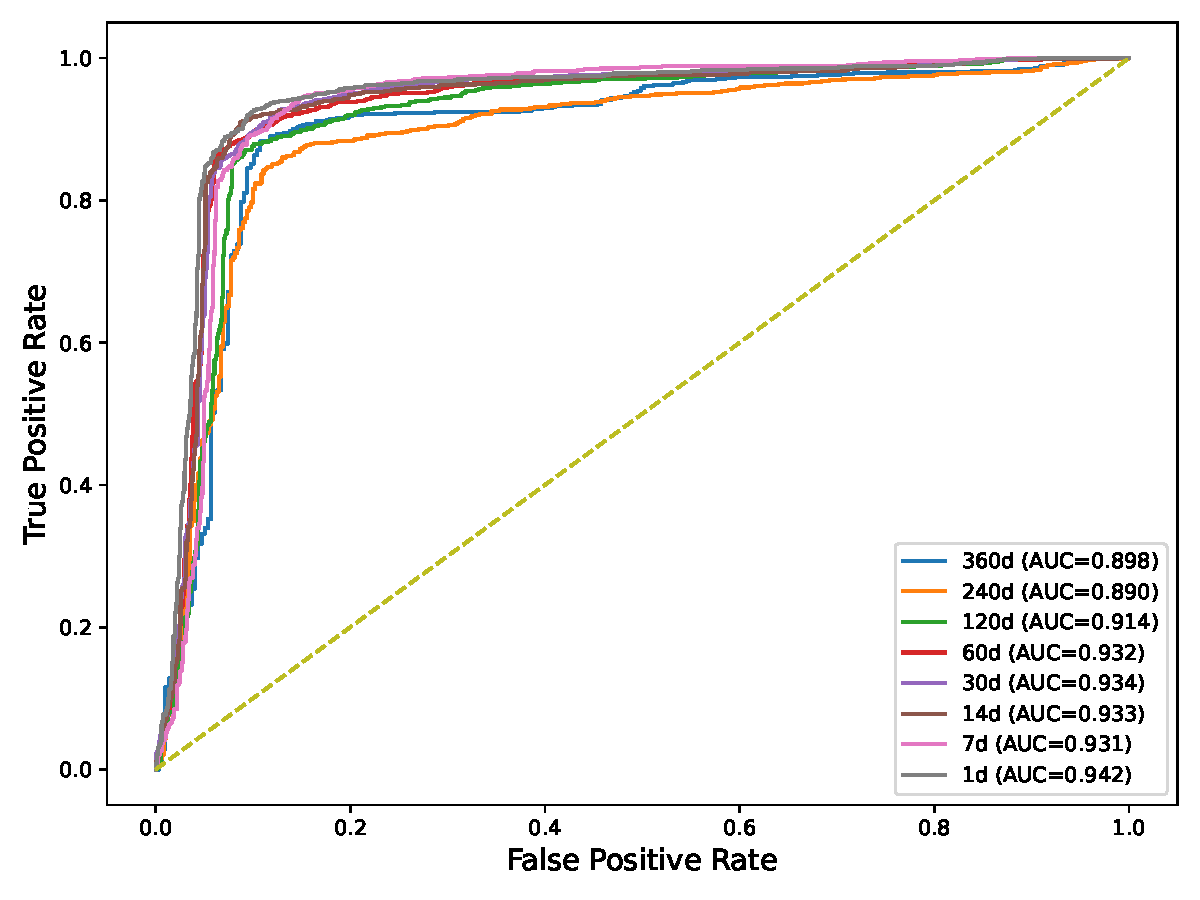
\includegraphics[width = 0.8\linewidth]{../Figures/log_roc.pdf}
	\caption{Logistic Models' AUCs}
	\label{fig:log-roc}
\end{figure}

Figure~\ref{fig:roi-beta}, similar to Figure~\ref{fig:roi-year}, simply depicts another way of examining the effect of campaign contributions on the probability of winning over time. 

\begin{figure}[H]
	\centering
	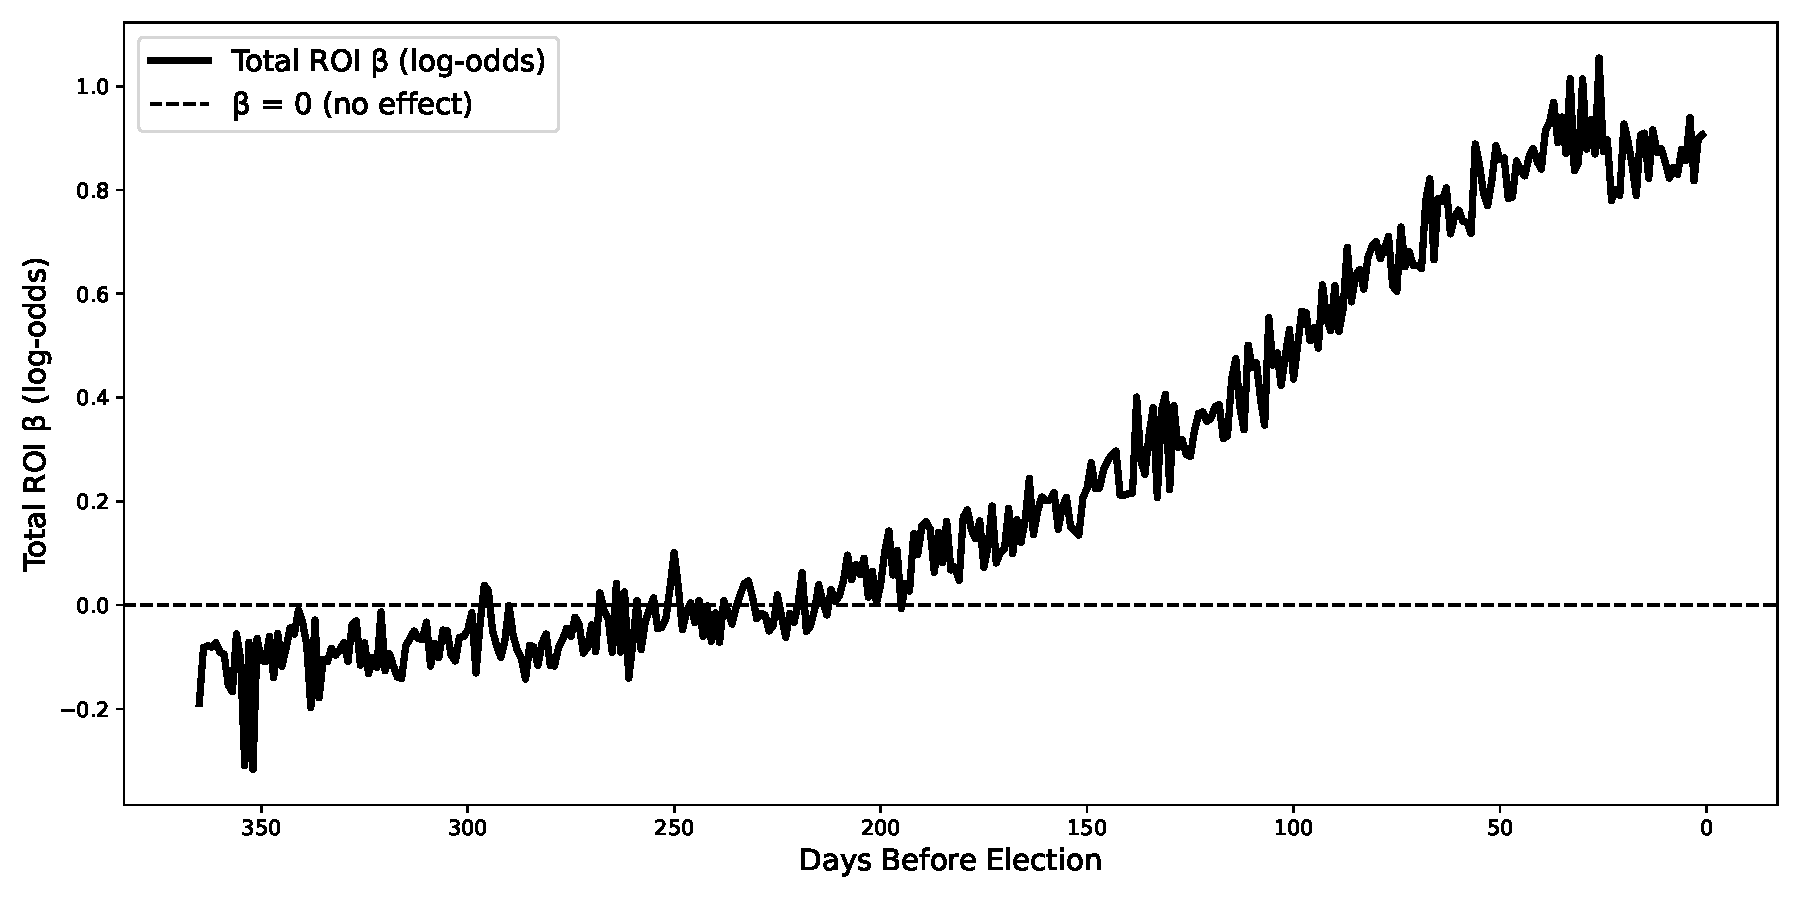
\includegraphics[width = 0.8\linewidth]{../Figures/roi_beta_over_time.pdf}
	\caption{Total (Raw) Return on Investment Trend a Year Prior to Election Day}
	\label{fig:roi-beta}
\end{figure}

Table~\ref{tab:gam-log-metrics} summarizes the GAM fits, showing AUC, accuracy, and recall for each cutoff.

\begin{table}[H]
	\centering
	\begin{tabular}{||c c c c c||}
\hline
Days & AUC & Accuracy & Recall (1) & Recall (0) \\
\hline\hline
360 & 0.914 & 0.896 & 0.939 & 0.724 \\
240 & 0.911 & 0.868 & 0.894 & 0.799 \\
120 & 0.938 & 0.887 & 0.891 & 0.882 \\
60 & 0.954 & 0.904 & 0.912 & 0.895 \\
30 & 0.960 & 0.904 & 0.909 & 0.898 \\
14 & 0.966 & 0.911 & 0.916 & 0.905 \\
7 & 0.963 & 0.909 & 0.928 & 0.887 \\
1 & 0.965 & 0.915 & 0.917 & 0.912 \\
\hline
\end{tabular}

	\caption{GAM Logistic Performance by Cutoff}
	\label{tab:gam-log-metrics}
\end{table}

Figure~\ref{fig:gam-or} depicts the odds-ratio trend over time using the logistic GAM.

\begin{figure}[H]
	\centering
	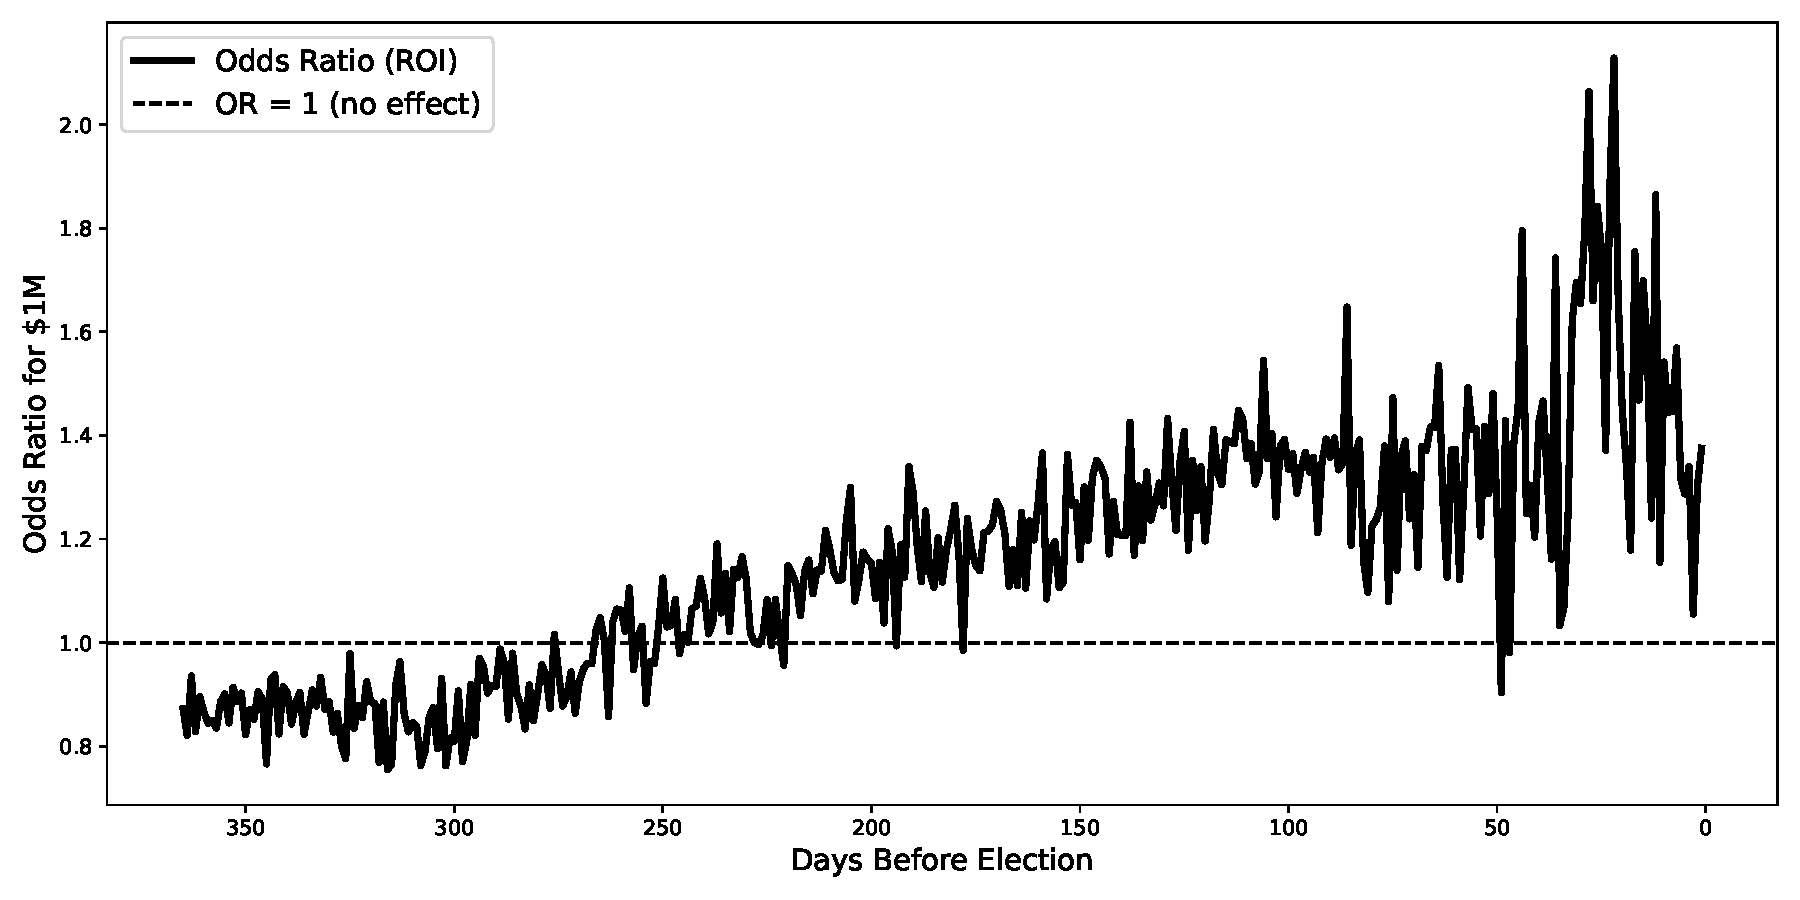
\includegraphics[width = 0.8\linewidth]{../Figures/gam_roi_over_time.pdf}
	\caption {GAM Total (Odds-Ratio) ROI Trend a Year Prior to Election Day}
	\label{fig:gam-or}
\end{figure}

Figure~\ref{fig:gam-roc} depicts the AUC achieved by the GAM logistic regression for each cutoff.

\begin{figure}[H]
	\centering
	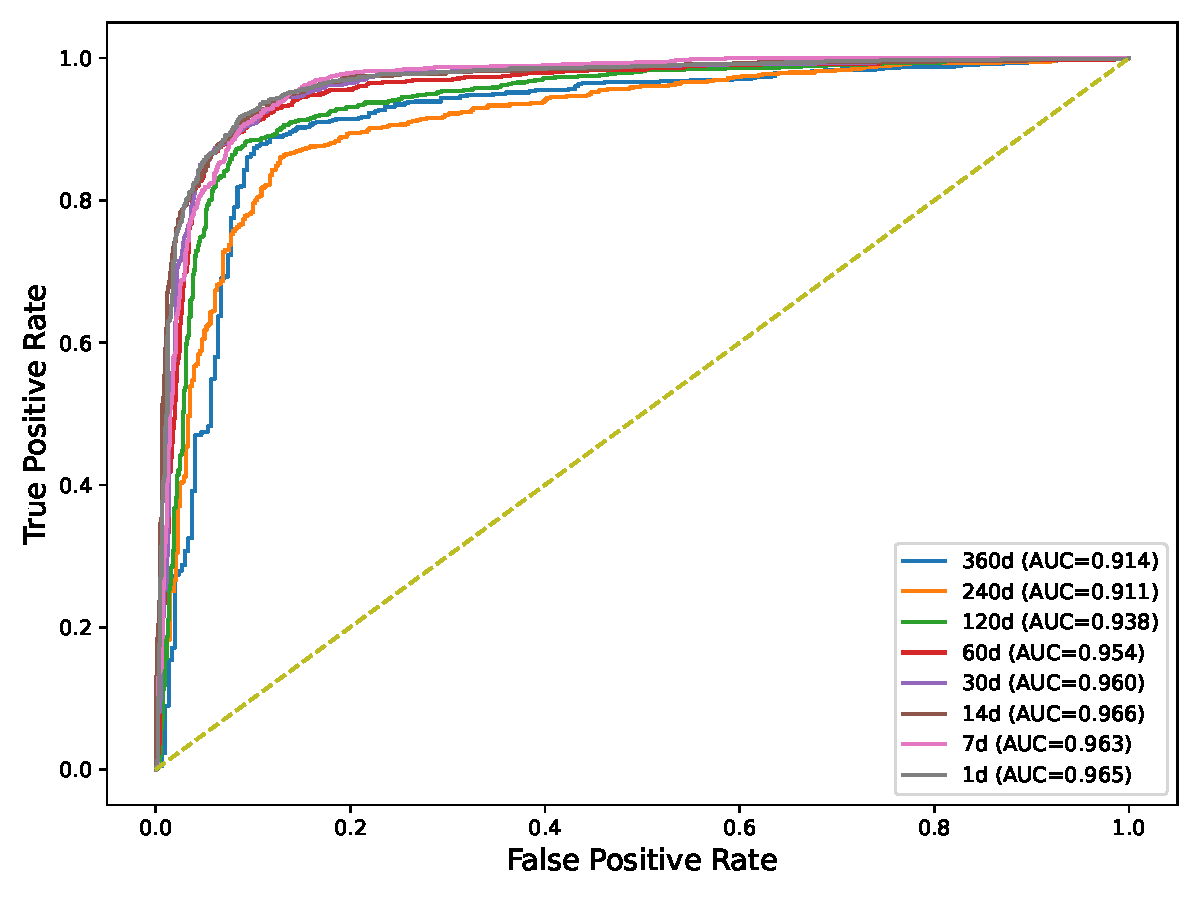
\includegraphics[width = 0.8\linewidth]{../Figures/gam_log_roc.pdf}
	\caption{Logistic GAM's AUCs}
	\label{fig:gam-roc}
\end{figure}

In Table~\ref{tab:ols-metrics}, I collect out-of-sample performance metrics ($R^2$, RMSE, MAE) and 5-fold CV $R^2$ for each cutoff from the simple least-squares models, while Table~\ref{tab:reg-r2} offers the regularized $R^2$ results and $\alpha$ given the better regularization technique (Ridge or LASSO).

\begin{table}[H]
	\centering
	\begin{minipage}{0.48\textwidth}
		\centering
		\begin{tabular}{||c c c c c||}
\hline
Days & $R^2$ & CV $R^2$ & RMSE & MAE \\
\hline\hline
360 & 0.410 & 0.393 & 13.672 & 9.715 \\
240 & 0.468 & 0.461 & 14.343 & 10.185 \\
120 & 0.555 & 0.560 & 14.372 & 10.208 \\
60 & 0.580 & 0.585 & 14.232 & 10.135 \\
30 & 0.587 & 0.596 & 14.168 & 9.980 \\
14 & 0.603 & 0.599 & 13.899 & 9.837 \\
7 & 0.609 & 0.601 & 13.926 & 9.987 \\
1 & 0.595 & 0.601 & 14.163 & 10.157 \\
\hline
\end{tabular}

		\caption{Least-Squares Regression Performance by Cutoff}
		\label{tab:ols-metrics}
	\end{minipage}\hfill
	\begin{minipage}{0.48\textwidth}
		\centering
		\begin{tabular}{||c c c||}
\hline
Days & Best Model ($\alpha$) & $R^2$ \\
\hline\hline
360 & RidgeCV (100.0000) & 0.410 \\
240 & RidgeCV (100.0000) & 0.468 \\
120 & LassoCV (0.1000) & 0.556 \\
60 & RidgeCV (17.7828) & 0.580 \\
30 & LassoCV (0.0316) & 0.588 \\
14 & LassoCV (0.0562) & 0.604 \\
7 & RidgeCV (31.6228) & 0.609 \\
1 & LassoCV (0.0562) & 0.595 \\
\hline
\end{tabular}

		\caption{Regularized $R^2$ for Each Cutoff}
		\label{tab:reg-r2}
	\end{minipage}
\end{table}

Table~\ref{tab:ho-metrics} reveals the hold-out performance for the linear GAM models.

\begin{table}[H]
	\centering
	\begin{tabular}{||c c c c||}
\hline
Days & HO $R^2$ & HO RMSE & HO MAE \\
\hline\hline
360 & 0.515 & 12.397 & 8.219 \\
240 & 0.532 & 13.452 & 9.051 \\
120 & 0.140 & 19.982 & 9.695 \\
60 & 0.522 & 15.178 & 9.454 \\
30 & 0.655 & 12.945 & 8.888 \\
14 & 0.695 & 12.180 & 8.583 \\
7 & 0.690 & 12.396 & 8.631 \\
1 & 0.693 & 12.322 & 8.728 \\
\hline
\end{tabular}

	\caption{GAM Linear Hold-Out Performance by Cutoff}
	\label{tab:ho-metrics}
\end{table}

Finally, the ROI of campaign contributions might also be expressed as elasticities, a unit-free measure of responsiveness. Raw elasticities measure the percent change in the probability of winning from a one percent increase in campaign contributions at a particular cutoff. Although not demonstrated here (due to the fact that I did not calculate the elasticities for each day across an entire election cycle), total spending over a political campaign may be thought of as a dynamic control/budget constraint problem. If total spending over the campaign is allocated across discrete time windows, it is natural that the sum of those period elasticities equal $1$: a one percent reallocation of total spending among time periods changes total spending by zero, so it cannot change the outcome in first order. Should anyone desire to calculate the ROI over an entire election cycle, this should be the result. 

For the sake of my goals, I calculated the raw elasticities for the arbitrary cutoffs I used throughout my research, as well as for the win-probability models across an entire year of campaigning. Because they are independent snapshots, they will \textit{not} sum to one; these elasticities are partial derivatives at particular time windows, so we do not get a partition of ``total elasticity.'' Furthermore, normalized elasticities tell one the share of total responsiveness that comes from spending at time $X$ (of the entire effect budget, what fraction is due to period $X$?). I also implemented these calculations, allowing one to compare periods directly on a common scale, leaving only the relative pattern over time. Altogether, this gives one another way to understand the ROI of campaign contributions.

\begin{table}[H]
	\centering
	\begin{minipage}{0.48\textwidth}
		\centering
		\begin{tabular}{||c c||}
\hline
Days & Elasticity \\
\hline\hline
360 & -0.012 \\
240 & -0.006 \\
120 & 0.177 \\
60 & 0.581 \\
30 & 1.129 \\
14 & 1.738 \\
7 & 1.683 \\
1 & 1.707 \\
\hline
\end{tabular}

		\caption{Raw Elasticities for MLE Logistic}
		\label{tab:log-elast}
	\end{minipage}\hfill
	\begin{minipage}{0.48\textwidth}
		\centering
		\begin{tabular}{||c c||}
\hline
Days & Elasticity \\
\hline\hline
360 & -0.029 \\
240 & 0.012 \\
120 & 0.084 \\
60 & -0.069 \\
30 & 0.370 \\
14 & 0.040 \\
7 & 0.406 \\
1 & 0.197 \\
\hline
\end{tabular}

		\caption{Raw Elasticities for GAM Logistic}
		\label{tab:log-gam-elast}
	\end{minipage}
\end{table}

\begin{table}[H]
	\centering
	\begin{minipage}{0.48\textwidth}
		\centering
		

		\caption{Raw Elasticities for Linear}
		\label{tab:lin-elast}
	\end{minipage}\hfill
	\begin{minipage}{0.48\textwidth}
		\centering
		\begin{tabular}{||c c||}
\hline
Days & Elasticity \\
\hline\hline
360 & -0.002 \\
240 & -0.001 \\
120 & 0.010 \\
60 & 0.020 \\
30 & 0.015 \\
14 & -0.004 \\
7 & -0.007 \\
1 & -0.006 \\
\hline
\end{tabular}

		\caption{Raw Elasticities for GAM Linear}
		\label{tab:lin-gam-elast}
	\end{minipage}
\end{table}

\begin{figure}[H]
	\centering
	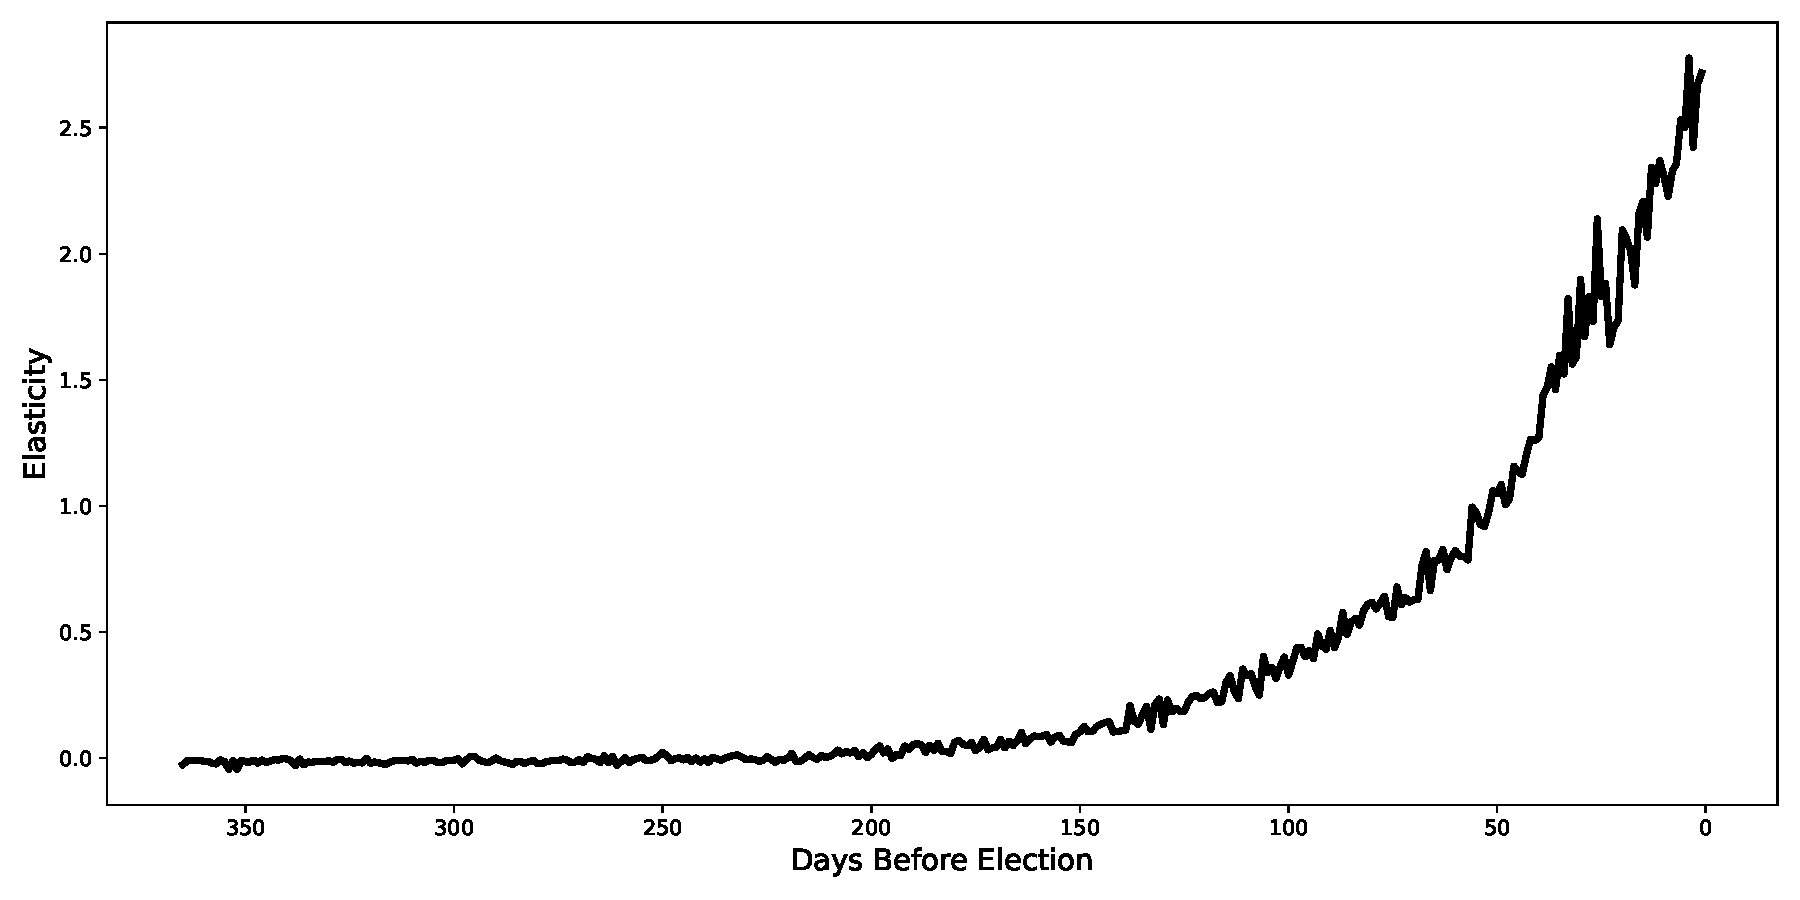
\includegraphics[width=0.8\linewidth]{../Figures/elasticity_over_time.pdf}
	\caption{MLE Logistic Model's Raw Elasticities over Time}
	\label{fig:log-e-time}
\end{figure}

\begin{figure}[H]
	\centering
	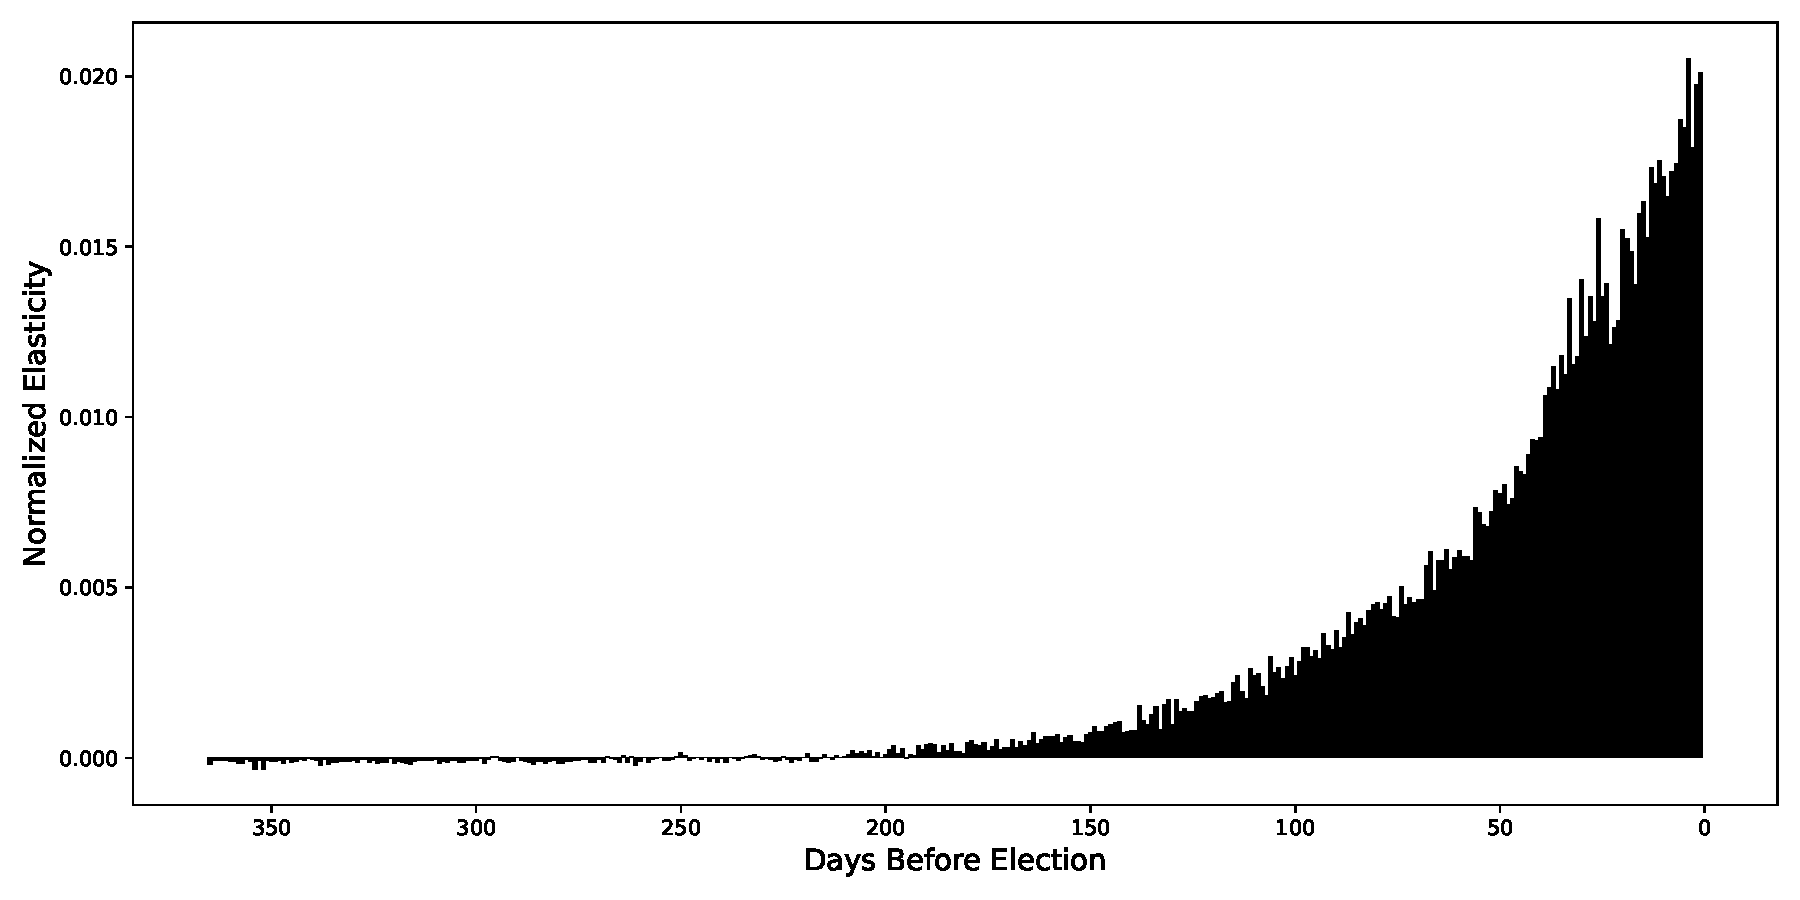
\includegraphics[width=0.8\linewidth]{../Figures/norm_elast_over_time.pdf}
	\caption{MLE Logistic Model's Normalized Elasticities over Time}
	\label{fig:log-norm-e-time}
\end{figure}

\begin{figure}[H]
	\centering
	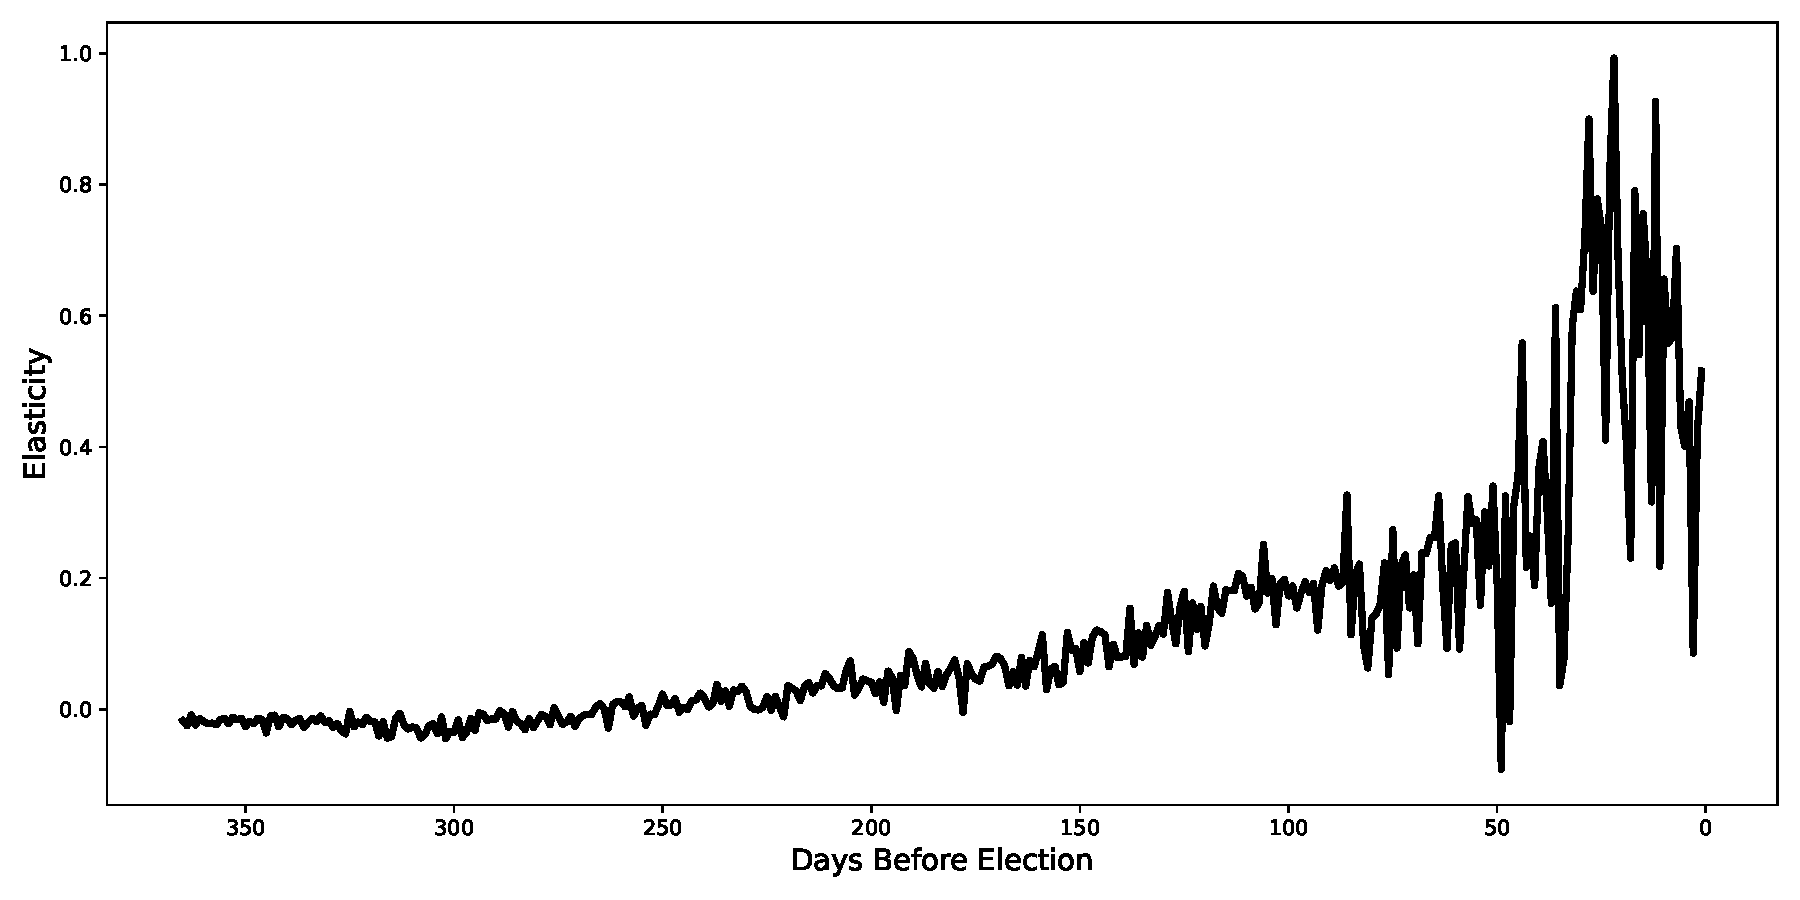
\includegraphics[width=0.8\linewidth]{../Figures/gam_elasticity_over_time.pdf}
	\caption{Logistic GAM's Raw Elasticities over Time}
	\label{fig:gam-log-e-time}
\end{figure}

\begin{figure}[H]
	\centering
	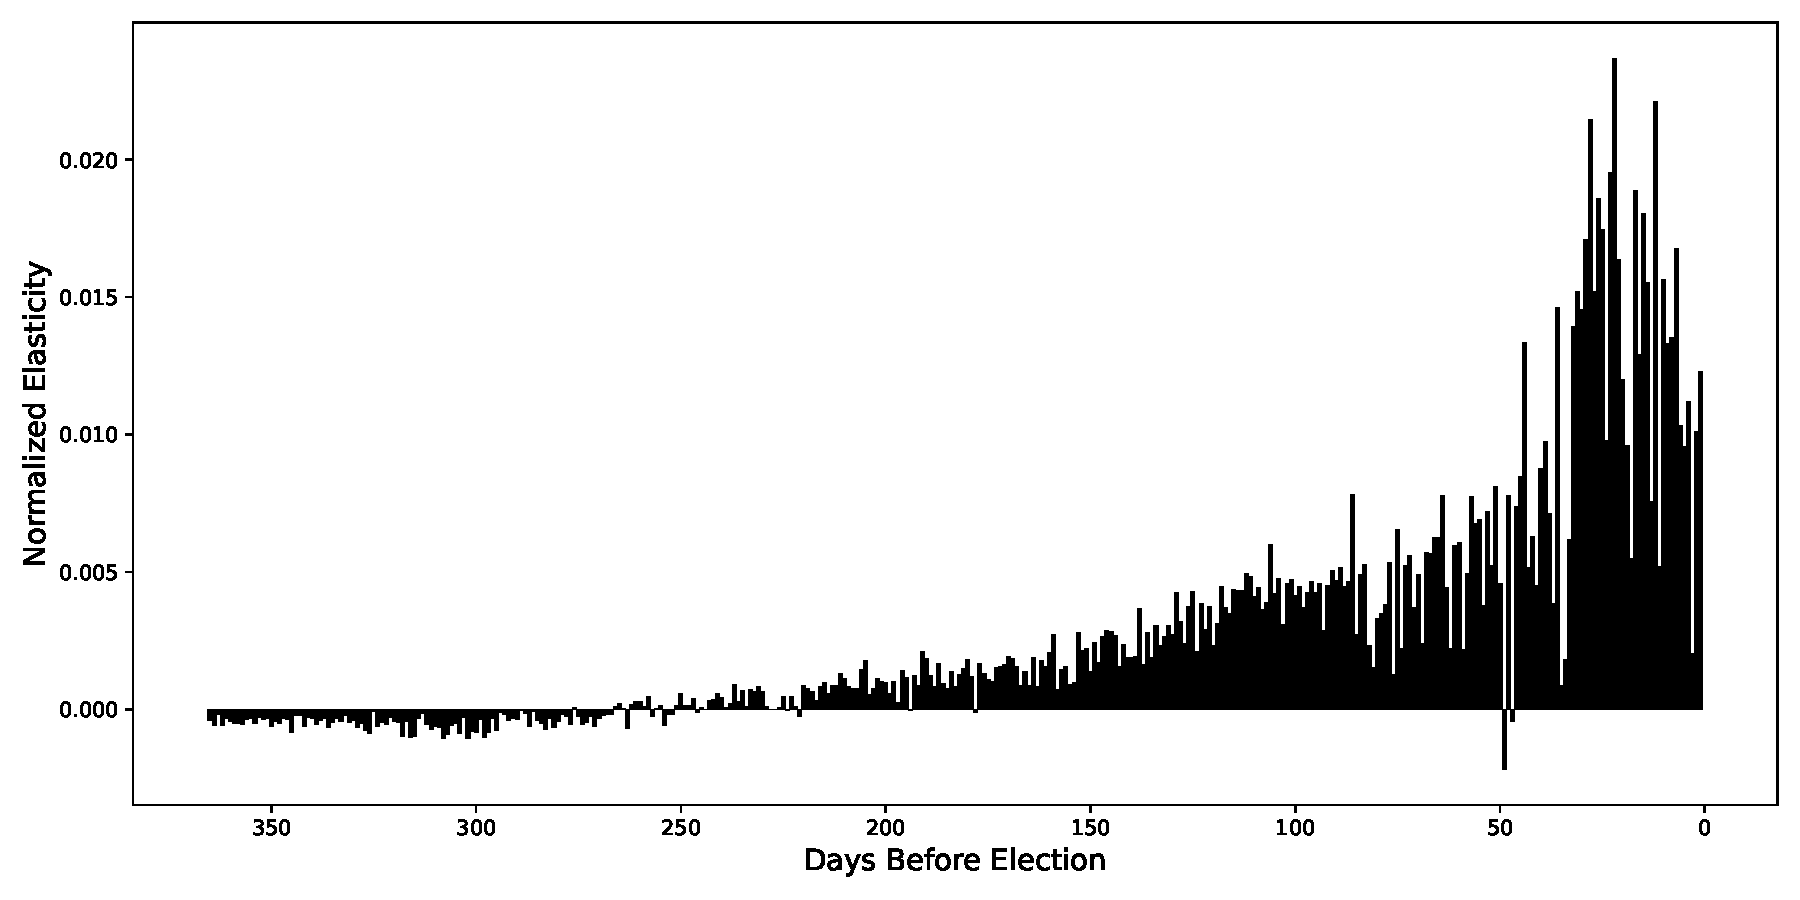
\includegraphics[width=0.8\linewidth]{../Figures/gam_norm_elast_over_time.pdf}
	\caption{Logistic GAM's Normalized Elasticities over Time}
	\label{fig:gam-log-norm-e-time}
\end{figure}



\newpage


\nocite{*}
\bibliographystyle{chicago}
\bibliography{../References/Paper}


\end{document}
